\documentclass[10pt, twoside]{article}



\usepackage{graphicx,color,epsfig}
\newcommand{\manualpath}{.}
\newcommand{\inputslocation}{\manualpath/inputs/}
\graphicspath{{\manualpath/diagrams/}{\manualpath/screencaps/}}

	
\usepackage{listings}
\lstset{language=}
\renewcommand\lstlistingname{File}
\renewcommand\lstlistlistingname{Files}
\lstset{numbers=none, numberstyle=\tiny, stepnumber=1, numbersep=5pt,captionpos=b,frame=single,breaklines=true,basicstyle=\small}




	
\usepackage{amsgen,amsmath,amstext,amsbsy,amsopn,amssymb}

\usepackage[dvipsnames]{xcolor}

\usepackage[colorlinks]{hyperref}
\hypersetup{
    colorlinks=true,       % false: boxed links; true: colored links
    linkcolor=Plum,          % color of internal links (change box color with linkbordercolor)
    citecolor=green,        % color of links to bibliography
    filecolor=magenta,      % color of file links
    urlcolor=cyan           % color of external links
}


\usepackage{float}

\usepackage[english]{babel}

\usepackage[left=1.25in,right=1.25in,top=1.25in,bottom=1.25in]{geometry} %
\usepackage[singlespacing]{setspace}%line spacing, set default to double

\usepackage{array}



\usepackage{makeidx}
\makeindex
	
	
\usepackage[format=plain,indention=.5cm,margin=10pt,font={small,singlespacing}]{caption}%custom captions.
\setlength{\parskip}{1em} %custom spacing between paragraphs 
	
	
	



% Alter some LaTeX defaults for better treatment of figures:
% See p.105 of "TeX Unbound" for suggested values.
% See pp. 199-200 of Lamport's "LaTeX" book for details.
%   General parameters, for ALL pages:
\renewcommand{\topfraction}{0.9}	% max fraction of floats at top
\renewcommand{\bottomfraction}{0.8}	% max fraction of floats at bottom
%   Parameters for TEXT pages (not float pages):
\setcounter{topnumber}{2}
\setcounter{bottomnumber}{2}
\setcounter{totalnumber}{4}     % 2 may work better
\setcounter{dbltopnumber}{2}    % for 2-column pages
\renewcommand{\dbltopfraction}{0.9}	% fit big float above 2-col. text
\renewcommand{\textfraction}{0.07}	% allow minimal text w. figs
%   Parameters for FLOAT pages (not text pages):
\renewcommand{\floatpagefraction}{0.7}	% require fuller float pages
% N.B.: floatpagefraction MUST be less than topfraction !!
\renewcommand{\dblfloatpagefraction}{0.7}	% require fuller float pages

% remember to use [htp] or [htpb] for placement

 

%scaling for the screen caps used in the manual
\newcommand{\screencapsize}{0.41}

%for inputting paramotopy input files
\newcommand{\File}[3]{
\begin{center}

\begin{minipage}{0.8\linewidth}
\lstinputlisting[
	caption={#1},
	label=file:#2]{\inputslocation#3}
\end{minipage}

\end{center}
}


%for inputting bertini real input files
\newcommand{\Filenobox}[3]{

\lstinputlisting[frame=none,
	breaklines=true,
	caption={#1},
	label=#2]{\inputslocation#3}

}

\usepackage{marginnote}
\renewcommand*{\marginfont}{\color{red}\sffamily\tiny}
\newcommand{\comment}[1]{\textcolor{red}{$\star$}\marginnote{#1}}



\usepackage[utf8]{inputenc}



\usepackage[acronym,toc,xindy]{glossaries}
\makeglossaries
\newglossaryentry{cmap}
{
    name=colormap,
    description={The set of colors that are used to vivify a figure in MATLAB},
    plural=colormaps
}
 
\newglossaryentry{dependent}
{
    name=dependency,
    description={A program (or programs) that need(s) to be installed in order for a different program to run},
    plural=dependencies
}
 
\newglossaryentry{rgbt} {
  name={RGB triple},
  description={A row vector with three columns with each entry ranging from zero to one used to identify a color},
  plural=RGB triples
}

\newglossaryentry{cpath}
{
    name=CPATH,
    description={A list of directories to be automatically searched for libraries, but are searched after all libraries tagged with \-I}
}

\newglossaryentry{lib}
{
    name=LIBRARY\_PATH,
    description={The value of LIBRARY\_PATH is a colon-separated list of directories, much like PATH. When configured as a native compiler, GCC tries the directories thus specified when searching for special linker files}
}
 
\newglossaryentry{ldlib}
{
    name=LD\_LIBRARY\_PATH,
    description={LD is the name of the unix linker. This environment variable is a colon-separated set of directories where libraries should be searched for first, before the standard set of directories and is useful when debugging a new library or using a nonstandard library for special purposes.}
} 

\newglossaryentry{path}
{
    name=PATH,
    description={The PATH environment variable is used by Cygwin applications as a list of directories to search for executable files to run.}
}

\newacronym[see={[Glossary:]{rgbt}}]{RGB}{RGB}{Red Green Blue color values\glsadd{rgbt}}

\newacronym{mpi}{MPI}{Message Passing Interface}

\newacronym{gmp}{GMP}{GNU Multiple Precision Arithmetic Library}

\newacronym{gcc}{GCC}{GNU C Compiler}

\newacronym{mpfr}{MPFR}{Multiple Precision Floating-Point Reliable}

\newacronym{mpc}{MPC}{GNU Multiple Precision Complex Library}

\newacronym{stl}{STL}{stereolithography}



\usepackage{multirow, bigstrut, booktabs}
\usepackage{longtable}
\usepackage{tabu}


\usepackage{titlesec}
\newcommand{\sectionbreak}{\clearpage}





\begin{document}
\pagestyle{front} 
	
	\pagenumbering{Alph}


\begin{titlepage}

	\begin{center}
	\vspace{2cm}
	{\Large Bertini\_real}

\vspace{\baselineskip}
	{\large Software for Real Algebraic Sets}



	{\large A Comprehensive Guide}	

	\vspace{3cm}
	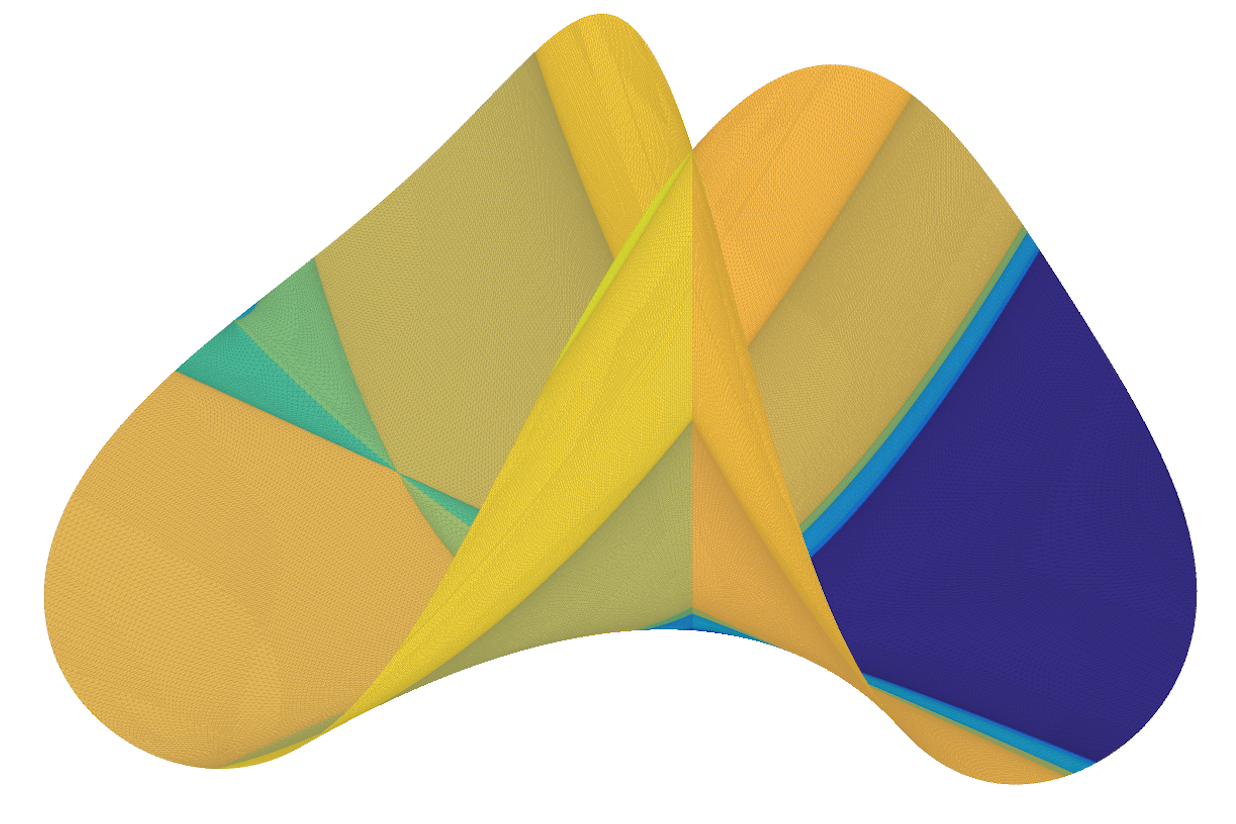
\includegraphics[width=0.75\linewidth]{whitney_ss.png}
	\end{center}

	\vfill

	\begin{minipage}{\linewidth}

	\begin{minipage}{0.4\linewidth}
	\centering
	This manual compiled \today \\
	\copyright 2014--\the\year\ Dani Brake
	\end{minipage}
	\hfill
	\begin{minipage}{0.4\linewidth}
	\centering Manual written by \vspace{\baselineskip}
	\\  Dani Brake \\ Pierce Cunneen \\ Elizabeth Sudkamp \\ Christopher Lembo
	\end{minipage}

	\end{minipage}

	

\end{titlepage}

\afterpage{\blankpage}

\pagenumbering{roman} 
	\setcounter{page}{1}
\begingroup\setlength{\parskip}{0pt plus .1pt}
	\tableofcontents
	\newpage
\endgroup



\pagestyle{main} 
\pagenumbering{arabic} 
	\setcounter{page}{1}
\setlength{\parskip}{1em plus 0.1em minus 0.1em} %custom spacing between paragraphs 

\section{Introduction}


Welcome to Bertini\_real, software for real algebraic geometry.  This manual is intended to help the user operate this piece of numerical software, to obtain useful and high-quality results from decomposing real algebraic curves and surfaces.

Bertini\_real is compiled software, links against a parallel version of Bertini 1 compiled as a library ({\tt libbertini-parallel}, and requires Matlab and the Symbolic Computation toolbox.  It also requires several other libraries, including a few from Boost, and an installation of MPI.  All libraries should be compiled using the same compilers and dependent libraries.  



\subsection{About this manual}
The purpose of this manual is to provide a robust, orderly, and easy to understand instructions on how to use Bertini\_real. This manual has three roles: it first serves as a description of what Bertini\_real is, followed by instructions on Bertini\_real's installation on Mac, Linux, and PC operating systems, and finally as a general reference manual for Bertini\_real.
	
This manual is here to help guide a user through the installation process, as well as act as the user's manual for Bertini\_real. If there is a section that might not be entirely clear, or is confusing to a reader, please contact us (see below for contact information), and we will try to resolve the problem. Such feedback is welcome!


\subsection{Bertini\_real product description}
	Bertini\_real is an implementation of several numerical algorithms \cite{lu2007finding,besana2013cell}, to decompose the real part of a complex curve or surface in any (tractible) number of variables.
	Some of the important features of Bertini\_real include :
\begin{itemize}
\item It is a command line program for numerically decomposing the real portion of a one- or two- dimensional complex irreducible algebraic  set in any reasonable number of variables.
\item It seeks to automate the visualization and computation of algebraic curves and surface.
\end{itemize}



\subsection{Where Bertini\_real can be found}
		
	The tarball for Bertini\_real can be downloaded at \href{http://www.bertinireal.com/download.html}{Bertini\_real.com}. 
	The visualization codes for MATLAB, they can be found at \href{https://github.com/ofloveandhate/bertini_real/tree/master/matlab_codes}{GitHub}.


	\subsection{Who is developing Bertini\_real?}
	Bertini\_real is under ongoing development by the development team, which consists of Dani Brake (University of Notre Dame), Daniel Bates (Colorado State University), Jonathan Hauenstein (University of Notre Dame), Wenrui Hao (Penn State), Andrew Sommese (University of Notre Dame), Charles Wampler (General Motors. R\&D), and Pierce Cunneen (University of Notre Dame)

	This manual was written by Dani Brake, Pierce Cunneen, Chris Lembo, and Elizabeth Sudkamp.


\subsection{Contact}
\label{sec:contact}

Dani Brake: \href{mailto:danielthebrake@gmail.com}{danielthebrake@gmail.com} -- Main implementer\\
Daniel Bates: \href{mailto:bates@math.colostate.edu}{bates@math.colostate.edu} -- Advisory \\
Jonathan Hauenstein: \href{mailto:hauenstein.edu}{hauenstein.edu} -- Advisory\\
Wenrui Hao: \href{mailto:hao.50@mbi.osu.edu}{hao.50@mbi.osu.edu} -- Advisory\\
Andrew Sommese: \href{mailto:sommese@nd.edu}{sommese@nd.edu} -- Advisory\\
Charles Wampler: \href{mailto:charles.w.wampler@gm.com}{charles.w.wampler@gm.com} -- Advisory\\
Pierce Cuneen: \href{mailto:pcuneen@nd.edu}{pcuneen@nd.edu} -- Users manual \\
Elizabeth Sudkamp: \href{mailto:esudkamp@nd.edu}{esudkamp@nd.edu} -- Users manual
% FUTURE CONTRIBUTORS, please add your name to both the 'Who is developing Bertini_real' section, as well as put in your contact email.

\subsection{Acknowledgements}

The development of Bertini\_real has been supported generously by a number of sources, including 
\begin{itemize}[noitemsep]
\item the Vincent J. and Annamarie Duncan Professor of Mathematics, at the University of Notre Dame, 
\item the University of Notre Dame, 
\item the National Science Foundation grants DMS-1025564 , DMS-1115668, and DMS-1262428, 
\item the Air Force Office of Scientific Research grant FA8650-13-1-7317, 
\item Mathematical Biosciences Institute, 
\item the Sloan Research Fellowship, 
\item the Army Young Investigators Project, and 
\item the Defense Advanced Research Projects Agency Young Faculty Award.
\end{itemize}

Finally, funding for shared facilities used in this research was provided by the Division of Computer and Network Systems: an NSF grant under award number CNS-0923386.




\subsection*{Disclaimer}

Any opinions, findings, and conclusions or recommendations expressed in this material are those of the author(s) and do not necessarily reflect the views of the National Science Foundation or any other organization.


\section{Quick Summary}
\label{sec:started}

Here's a super brief description of how to get and use this software:

Bertini\_real can be downloaded from \url{http://bertinireal.com/download.html}, or cloned from \href{https://github.com/ofloveandhate/bertini_real}{its Github repo}.  Use of Bertini\_real depends on Bertini, which itself has several important dependencies (see section \ref{sec:installation})
Once installed, you can run Bertini\_real on an input file from the command line. After navigating to the working directory of the input file, the flow of Bertini\_real is as follows:
\begin{enumerate}
\item Open Command Terminal. 
\item Run Bertini on an input file using the \texttt{tracktype:1} setting. This is done by typing in the command line: \texttt{bertini} with an input file named \texttt{input}. Bertini will produce a Numerical Irreducible Decomposition that will be used by Bertini\_real.
\item Run Bertini\_real on the same input file. Similarly, just type \texttt{bertini\_real} in the command line. Bertini\_real will provide a cellular decomposition of the real portion of a one- or two- dimensional complex algebraic set.
\item Visualize the results of Bertini\_real in Matlab. Enter Matlab and call \texttt{gather\_br\_samples}, which parses the output results of  into a .mat file, and then call \texttt{bertini\_real\_plotter}, which will plot the curve or surface in Matlab.  Please note that the Matlab executable must be on the path to the input file for Bertini\_real to run). 
\end{enumerate}





\section{Input Files}

\label{sec:input}


The instructions provided go through how to create input files, run these files through Bertini and Bertini\_real, and view a graphical representation of the results using MATLAB. Most of this information about Bertini, its input files, and syntax will be taken or paraphrased from the slightly-out-of-date Bertini User's Manual, which can be read \href{https://bertini.nd.edu/BertiniUsersManual.pdf}{here}. 


The \texttt{input} file has two parts, grouped as follows (where the \% symbol is the comment character in the \texttt{input} file, as usual):

\begin{center}\begin{minipage}{0.9\linewidth}

\begin{lstlisting}[language=c++, caption=Adapted from \cite{BM13}, captionpos=b]
CONFIG
% Lists of configuration settings (optional)
tracktype:1; % needed in order to run Bertini_real
END;
INPUT
% Symbol declarations
% Optional assignments (parameters, constants, etc.)
% Function definitions
END;
\end{lstlisting}
\end{minipage}\end{center}

The upper portion of the file consists of a list of configuration settings. Any configuration that is not listed in the \texttt{input} file will be set to its default value. A table of all configuration settings that may be changed, along with their default settings and acceptable ranges, may be found in the Appendix.\par
The syntax for the configuration lines is straightforward. It consists of the name of the setting (in all caps), followed by a colon, a space, the setting, and a semicolon. For example, to change the tracking type to 1 (the default is 0), simply include the following line in the \texttt{CONFIG} portion of the \texttt{input} file:

\begin{center}\begin{minipage}{0.9\linewidth}

\begin{lstlisting}[language=c++, caption=Adapted from \cite{BM13}, captionpos=b]
TRACKTYPE: 1;
\end{lstlisting}
\end{minipage}\end{center}

The lower portion of the \texttt{input} file begins with a list of symbol declarations (for the variables, functions, constants, and so on). All such declarations have the same format:
\begin{center}\begin{minipage}{0.9\linewidth}

\begin{lstlisting}[language=c++, caption=Adapted from \cite{BM13}, captionpos=b]
KEYWORD a1, a2, a3;
\end{lstlisting}
\end{minipage}\end{center}

where \texttt{KEYWORD} depends upon the type of declaration. All symbols used in the \texttt{input} file must be declared, with the exception of subfunctions. Here are details regarding each type of symbol that may be used in the input file:
\begin{itemize}

\item{FUNCTIONS:}
Regardless of the type of run, all functions must be named, and the names must be declared using the keyword \texttt{function}. Also, the functions must be defined in the same order that they were declared.

\item{VARIABLES}
In all cases except user-defined homotopies, the variables are listed by group with one group per line, with each line beginning with either the keyword \texttt{variable\_group} (for complex variable groups against which the polynomials have not been homogenized) or the keyword \texttt{hom\_variable\_group} (for variable groups against which the polynomials have been homogenized).
 Note that the user must choose one type of variable group for the entire input file, i.e., mixing of variable groups is not allowed in this release of Bertini. Also, only one variable group may be used for a positive-dimensional run. For example, if there are two
 nonhomogenized variable groups, the appropriate syntax would be
\begin{center}\begin{minipage}{0.9\linewidth}

\begin{lstlisting}[language=c++, caption=Adapted from \cite{BM13}, captionpos=b]
variable_group z1, z2;
variable_group z3;
\end{lstlisting}
\end{minipage}\end{center}

In the case of user-defined homotopies, the keyword is \texttt{variable}, and all variables should be defined in the same line.

\item{PATHVARIABLES:}
The pathvariable, often denoted by the letter “t”, is the independent variable that is controlled during homotopy continuation. In Bertini, the homotopy always moves from the start system at $t = 1$ to the target system at $t = 0$. A pathvariable must be declared in the \texttt{input} file \textbf{ONLY} if the user is specifying the entire homotopy (i.e., \texttt{USERHOMOTOPY} is set to 1). In that case, it is also necessary to declare at least one parameter, as described in the next item. The keyword for pathvariables is \texttt{pathvariable}.

\item{PARAMETERS:}
Homotopy continuation relies on the ability to cast a given polynomial system as a member of a parameterized family of polynomial systems. Such parameterized families (especially those which occur naturally) constitute one of the powerful advantages numerical methods in algebraic geometry have over symbolic methods. Sometimes there is only one parameter involved, but sometimes there are several. Please note, though, that user-defined parameters should be used only in the case of user-defined homotopies. Regardless of the number of parameters, each parameter depends directly upon the pathvariable. As a result, the user must both declare each parameter and assign to it an expression depending only upon the pathvariable to it. Here is an example:
\begin{center}\begin{minipage}{0.9\linewidth}

\begin{lstlisting}[language=c++, caption=Adapted from \cite{BM13}, captionpos=b]
...
parameter p1, p2;
...
p1 = t^2;
p2 = t^3;
...
\end{lstlisting}
\end{minipage}\end{center}

For technical reasons, in the case of a user-provided homotopy, Bertini always assumes that there is at least one parameter (even if there is no apparent need for one). In the case that the user wishes to build a homotopy depending only upon the pathvariable, it is necessary to declare a parameter, set it to the pathvariable in the assignments section, and then to use only that parameter (and \textbf{NOT} the pathvariable) in the functions. Here is an example:
\begin{center}\begin{minipage}{0.9\linewidth}

\begin{lstlisting}[language=c++, caption=Adapted from \cite{BM13}, captionpos=b]
...
pathvariable t;
parameter s;
...
s=t;
...
\end{lstlisting}
\end{minipage}\end{center}

No parameters should appear in the \texttt{input} file unless the homotopy is defined by the user, and the pathvariable should never appear explicitly in any homotopy function.

\item{CONSTANTS:}
Bertini will accept numbers in either standard notation (e.g., 3.14159 or 0.0023) or scientific notation (e.g., 3.14159e1 or 2.3e-3). No decimal point is needed in the case of an integer. To define complex numbers, simply use the reserved symbol I for $\sqrt{-1}$, e.g., \texttt{1.35 + 0.98*I}. Please note that the multiplication symbol * is always necessary, i.e. concatenation does not
 mean anything to Bertini. Since it is sometimes useful to have constants gathered in one location (rather than scattered
 throughout the functions), Bertini has a \texttt{constant} type. If a constant type is to be used, it must be both declared and assigned to. Here is an example:
\begin{center}\begin{minipage}{0.9\linewidth}

\begin{lstlisting}[language=c++, caption=Adapted from \cite{BM13}, captionpos=b]
...
g1 = 1.25;
g2 = 0.75 - 1.13*I;
...
\end{lstlisting}
\end{minipage}\end{center}

Bertini will read in all provided digits and will make use of as many as possible in computations, depending on the working precision level. If the working precision level exceeds the number of digits provided for a particular number, all further digits are assumed to be
 0 (i.e., the input is always assumed to be exact). This seems to be the natural, accepted implementation choice, but it could cause difficulty if the user truncates coefficients without realizing the impact of this action on the corresponding algebraic set.

\item{SUBFUNCTIONS:}
Redundant subexpressions are common in polynomial systems coming from applications. For example, the subexpression \texttt{x\string^ 2 + 1.0} may appear in each of ten polynomials. One of Bertini’s advantages is that it allows for the use of subfunctions. To use a subfunction, simply choose a symbol, assign the expression to the symbol, and then use it in the functions. There is no need to declare subfunctions (and no way to do so anyway).

\begin{center}\begin{minipage}{0.9\linewidth}
\begin{lstlisting}[language=c++, caption=Adapted from \cite{BM13}, captionpos=b]
...
V = x/2 + 1.0;
...
f1 = 2*V^2 + 4.0;
...
\end{lstlisting}
\end{minipage}\end{center}

\item{SIN, COS, PI, AND EXP:}
Starting with Bertini v1.2, the sine function sin, cosine function cos and exponential function exp are built into Bertini. Additionally, Bertini uses \texttt{Pi} for the constant $\pi$. To avoid confusion with scientific notation, the constant \textit{e} is not specifically built in Bertini, but the user can define their own constant and set it equal to \texttt{exp(1)}, as shown below.
\begin{center}\begin{minipage}{0.9\linewidth}

\begin{lstlisting}[language=c++, caption=Adapted from \cite{BM13}, captionpos=b]
...
constant EN; % Euler's number e
EN = exp(1);
...
\end{lstlisting}
\end{minipage}\end{center}

It is important to note that Bertini will return an error if the argument of \texttt{sin}, \texttt{cos}, or \texttt{exp} depends upon a variable when trying to solve a polynomial system. There is no such restriction for user-provided homotopies.
\end{itemize}


\subsection{On Bertini input syntax}
Common complaints about Bertini are that (a) the parser that reads in the input is very picky and (b) the error messages are often to general. The development team agrees and will continue to work on this (especially during an upcoming complete rewrite). In the meantime, here is a list of syntax rules that are commonly broken, resulting in syntax errors:

\begin{itemize}
\item All lines (except \texttt{CONFIG} and \texttt{INPUT}, if used) must end with a semicolon.
\item Bertini is case-sensitive.
\item The symbol for $\sqrt{-1}$ is \texttt{I}, not \texttt{i}. If you prefer to use \texttt{i}, you may define \texttt{i} as a subfunction by
including the statement \texttt{i = I;}.
\item In scientific notation, the base is represented by \texttt{e} or {\tt E}, e.g., 2.2e-4. 
\item For multiplication, * is necessary (concatenation is not enough).
\item Exponentiation is designated by \string^.
\item All symbols except subfunctions must be declared prior to use.  You cannot combine declaration and definition, sadly.
\item No symbol can be declared twice. This error often occurs when copying and pasting in the
creation of the input file.
\item A pathvariable and at least one parameter are needed for user-defined homotopies. Please
refer to the previous section for details.
\item White space (tabs, spaces, and new lines) is ignored.
\end{itemize}


\section{The Decomposition Algorithms}
\label{sec:algo}

This section of the manual describes, hopefully without too much techinical detail, the curve and surface decomposition algorithms.  The main academic paper on this is \cite{besana2013cell}, while the paper on Bertini\_real implementing it is \cite{BrN15}.  Two additional extended abstracts discussing it are \cite{Brake2014, On14}.

We invite you to play with the software and visualization routines, to experience these algorithms first-hand.  Danielle in particular thinks of these algorithms as implementations of the implicit function theorem.  Enjoy!


\subsection{Decomposing curves}
\label{sec:algo_curve}



Decomposing an algebraic curve numerically can be summarized easily in six steps:
%
\begin{enumerate}[noitemsep]
\item Compute critical points
\item Intersect with bounding object
\item Slice at projection interval midpoints
\item Connect the dots
\item Merge [optional]
\item Sample [optional]
\end{enumerate}

A curve is decomposed with respect to projection onto a (randomly chosen) real linear projection, $\pi_0(x)$.


What does it mean to decompose a curve?  To turn compute a set of {\em edges} that describe the curve.  An edge is a 1-dimensional object, having two points as boundary, and a general point in the middle, together with a homotopy which can be used to track the midpoints between the boundary points.  Phew.  See Figure~\ref{fig:edge}.




\begin{figure}[H]
\begin{center}
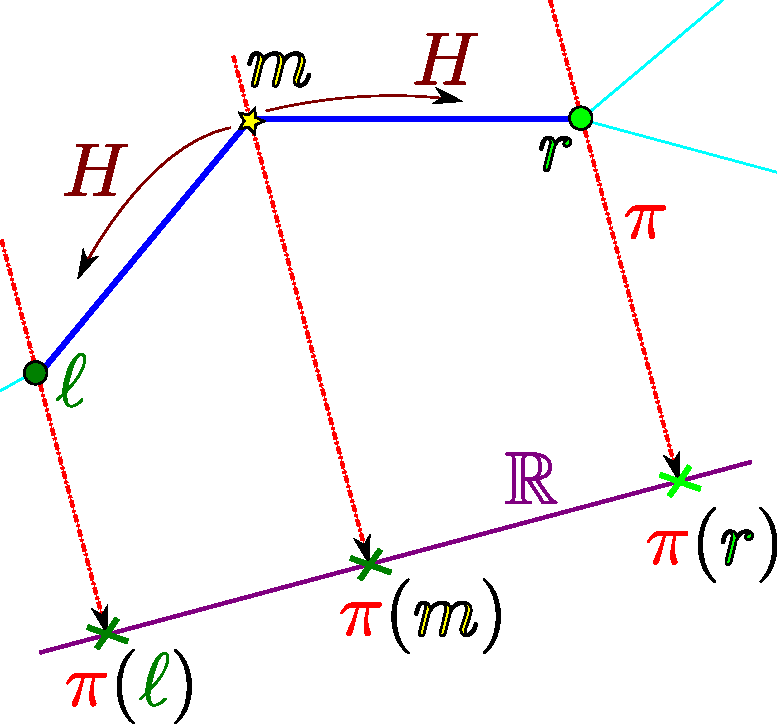
\includegraphics[width = 2in]{edge}
\caption{An edge, a 1-cell, as a component of a curve decomposition.}
\label{fig:edge}
\end{center}
\end{figure}


\subsubsection{Critical points}

Critical points of a curve satisfy the following system:
\begin{equation}
\begin{bmatrix}
f(x) \\
\textnormal{det} \begin{pmatrix} Jf(x) \\ J\pi_0 \end{pmatrix}
\end{bmatrix}  = 0. \label{eqn:curve_critpts}
\end{equation}
These points include singular points (trivially, and independently of projection).  This is solved by a 2-homogeneous regeneration procedure.


\subsubsection{Intersect with bounding object}

To capture the behaviour of the curve as it goes to $\infty$, we intersect the curve with a bounding object, and ignore all outside points.  In Bertini\_real, we use a sphere centered at the centroid of the critical points, with radius 3 times the distance to the furthest critical point.  The user can choose their own sphere of interest.


\subsubsection{Slice}


Let the set of critical points just computed be $\chi$.  Then, take $\pi_0(\chi)$, the set of critical projection values.  We slice at midpoints of projection intervals defined by this set.  This computes the set of midpoints for (unmerged) edges computed by the next step.


\subsubsection{Connect the dots}
\label{sec:connect_curve}


Connecting the dots for a curve simply means to track each midpoint to the left and right bounding critical projection values, and see what critical points match.  This forms an edge.  The homotopy 
\begin{equation}
(1-t)
\begin{bmatrix}
f(x) \\
\pi_0(x) - p_{c_j}
\end{bmatrix}
+t
\begin{bmatrix}
f(x) \\
\pi_0(x) - p_{m_i}
\end{bmatrix} = 0\label{eqn:projvalmove}
\end{equation}
is used.

Some midpoints may track to points in critical fibers which have not yet been previously computed.  In software, these are classified as {\em semicritical}.

\subsubsection{Merge [optional]}

Merging edges combines two edges which meet at a non-critical point.  These points occur when tracking midpoints toward critical projection values yields a new point, one in the fiber of a true critical point.  A simpler curve decomposition can be obtained by merging such edges.  There are times when merging is great (most of the time) and times when merging is not the right thing to do (some points in the surface decomposition algorithm).

Merging can be disabled when decomposing a curve in Bertini\_real with the {\tt -nomerge} flag.


\subsubsection{Sample [optional]}
Suffice it to say for now that a midpoint is tracked using \eqref{eqn:projvalmove} within the bounds of its edge, producing additional points on the edge.  
This section is described in much greater detail in Section~\ref{sec:sampler_curve}.   



















\subsection{Decomposing surfaces}
\label{sec:algo_surface}


Decomposing an algebraic surface numerically is similar to that of a curve, and can also be summarized in about six steps:
%
\begin{enumerate}[noitemsep]
\item Compute critical curves
\item Intersect with bounding object
\item Slice at projection interval midpoints.  The slices are curve decompositions
\item Connect the dots to form faces
\item Merge [optional]
\item Sample [optional]
\end{enumerate}


To decompose a surface is to compute a set of {\em faces}.  A face is a 2-cell, containing a set of bounding edges, and a general point in the middle, which can be tracked using a homotopy, staying within the boundary.  See Figure~\ref{fig:face}

\begin{figure}[H]
\begin{center}
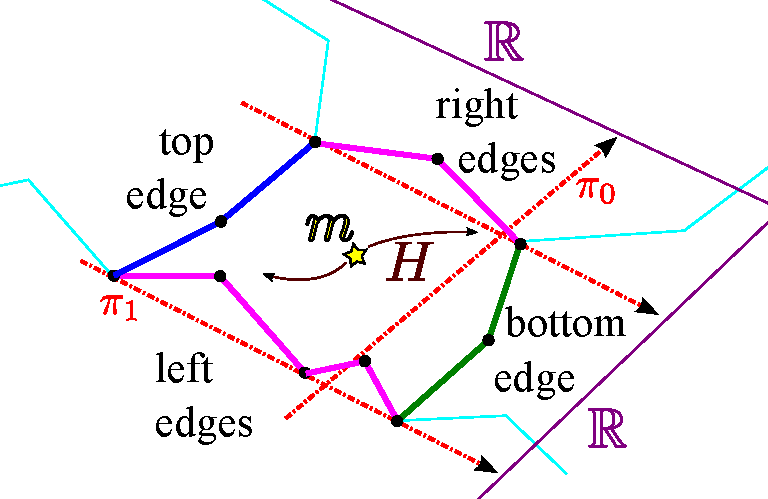
\includegraphics[width = 2in]{face}
\caption{A face, a 2-cell, as a component of a surface decomposition.  Its boundary consists of edges from curve decompositions.}
\label{fig:face}
\end{center}
\end{figure}

A surface is decomposed with respect to projection onto a pair of (randomly chosen) real linear projections, $\pi_0(x)$ and $\pi_1(x)$, together which may be referred to as $\pi(x)$.

\begin{figure}[H]
\begin{center}
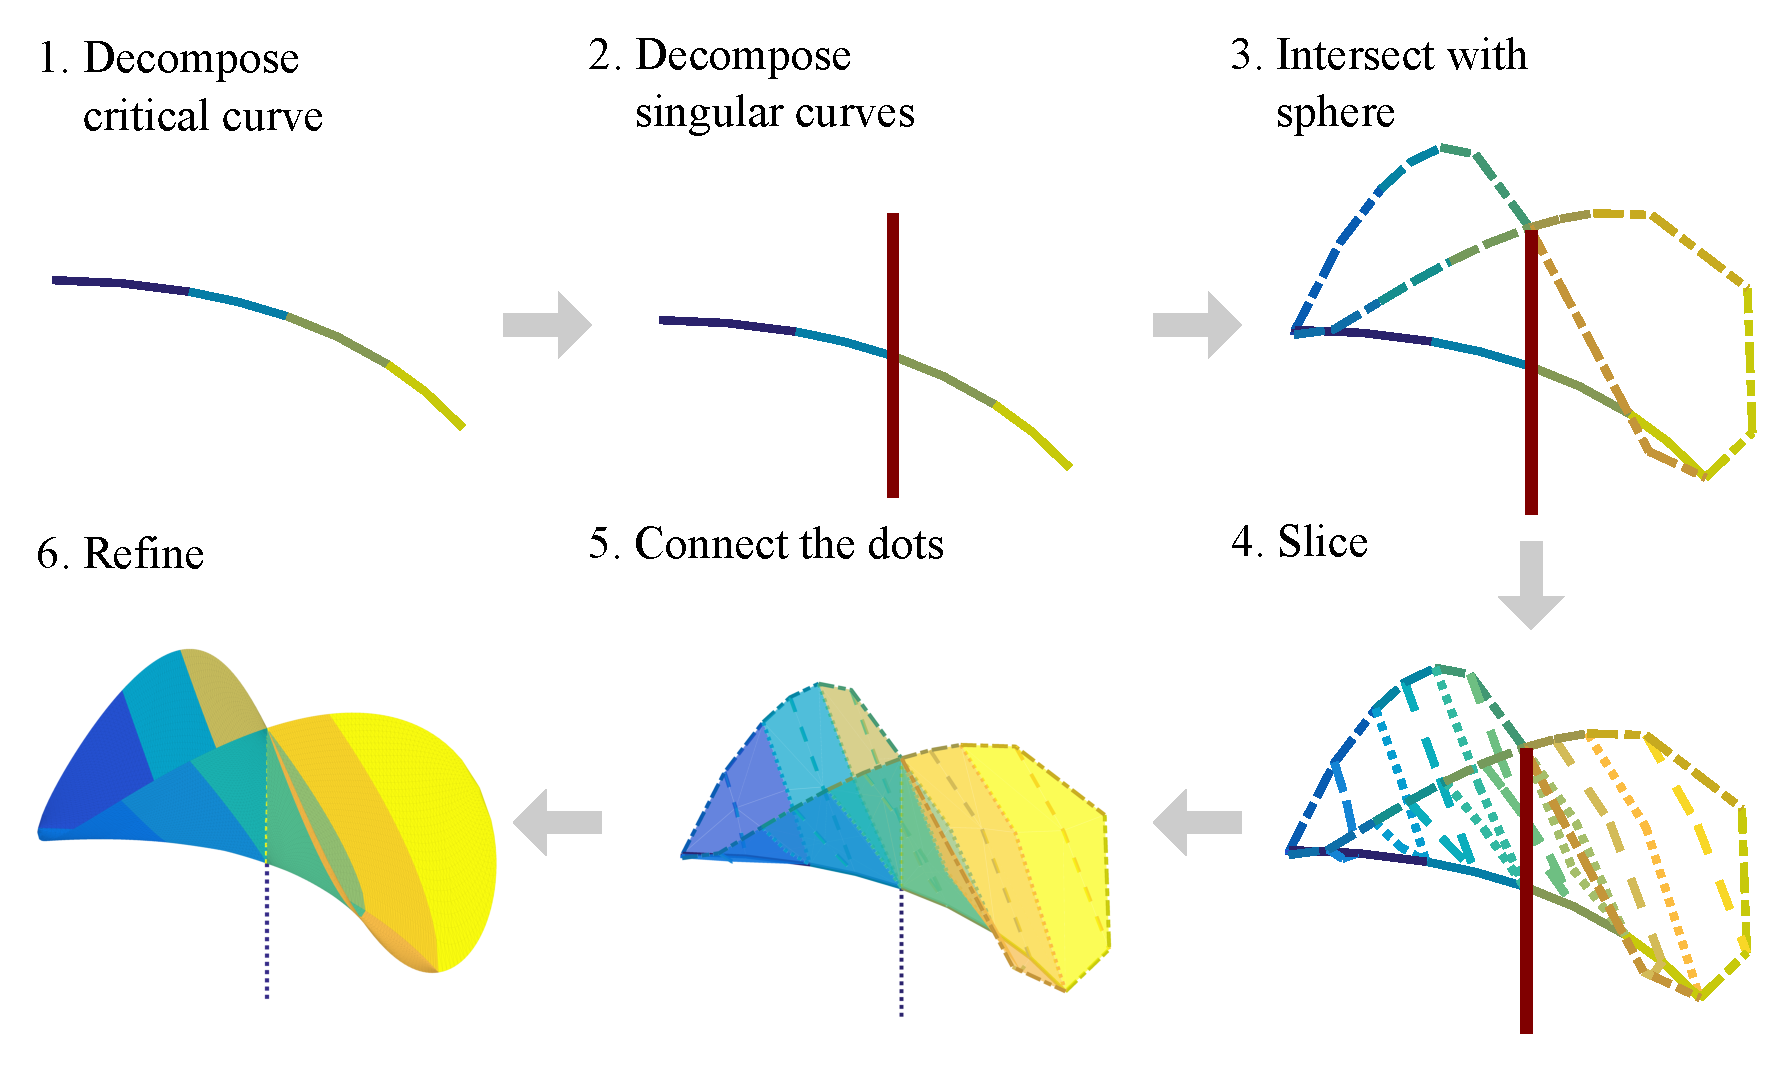
\includegraphics[width = 5in]{surface_method}
\caption{Numerical cellular decomposition of the Whitney Umbrella using Bertini\_real.}
\label{fig:decomposing_surface}
\end{center}
\end{figure}






\subsubsection{Critical curves}

Critical curves can be separated into two categories.  First, those which are an artifact of the projection being used to decompose.  Second, those which appear regardless of the projection.  In this manual and software, we refer to the former simply as the {\em non-singular critical curve} or simply {\em critical curve}, and the second as {\em singular curves}, although they both are formally part of the critical curve (and so is the bounding curve).


\paragraph{Nonsingular critical curve}

The non-singular critical curve satisfies this system, nonsingularly:
\begin{equation}\label{eqn:crit_curve}
    F(x) = \begin{bmatrix}
f(x) \\
\det \begin{pmatrix}
    Jf(x) \\
    J\pi_0 \\
    J\pi_1
            \end{pmatrix} \\
\end{bmatrix} = 0.
\end{equation}
In current implementation using Bertini1 as the homotopy engine, we use a symbolic engine to compute a new text Bertini input file.  There are several options for the symengine, described in Section~\ref{sec:running_br}.  A curve decomposition is run on this curve.  But first, we have to have {\em \bf all} of the critical points of all critical curves, including non-singular, singular, and bounding.


\paragraph{Singular curves}

Not every surface has singular curves, but many do.  Perhaps the easiest to see at first is the Whitney Umbrella.
\begin{equation}
f = x^2 - y^2 z = 0
\end{equation}
This equation describes a degree 3 surface.  The $z$-axis is singular.  Observe the Jacobian:
\begin{equation}
Jf = \begin{bmatrix}
2x & -2yz & -y^2
\end{bmatrix}
\end{equation}
On the $z$-axis, $x = y = 0$.  So, $Jf$ is singular.  Hence the determinant in \eqref{eqn:crit_curve} is $0$, which means the critical curve system is in some sense trivially satisfied.  What is needed here is to {\em deflate} the system.  This is accomplished in current implementation using {\em isosingular deflation} \cite{hauenstein2013isosingular}.  Basically, sub-determinants of the system are recursively added until the rank of the Jacobian stabilizes, where this rank is computed using a witness point for the component being deflated.

The singular curves are decomposed using the curve algorithm, after obtaining {\em all} critical points of {\em all} critical-like curves.

\subsubsection{Bounding curve}

To capture the behaviour of surfaces which are not closed or bounded, we intersect the surface with a bounding object.  The implemented type in Bertini\_real is sphere.  Initially, we had implemented a bounding box, and it was neat, but for higher dimensions, it meant doing more and more curve decompositions, with each of the $2N$ planes.  It got messy.  So, surfaces are used.  They are easier, because the entire bounding curve satisfies a single system, which is merely the original system supplemented with a single degree 2 equation -- that of the sphere.  It eases not only implementation but also runtime.

We compute the sphere automatically, after having computed the critical points of the critical and singular curves (but before decomposing them, for algorithmic reasons).  The sphere is centered at the centoid of all critical points, and its radius is arbitrarily chosen to be 3 times the distance from the center to the furthest critical point.  The user may also supply their own sphere of interest (See Section~\ref{sec:running_br}).




\subsubsection{Slice}


Having decomposed all formal parts of the critical curve, we slice the surface.  Where?  

Consider all critical points of all thus-far computed curves.  Call this set $\chi$.  Then we project onto the first projection coordinate, computing $\pi_0(\chi)$.  This set of values produces the critical slices.  Taking midpoints of all intervals defined by $\pi_0(\chi)$ defines the mid slices.  Each of these slices is computed using a regular curve decomposition.





\subsubsection{Connect the dots}
\label{sec:connect_surface}

This is a fun piece of the puzzle.  In this part of the algorithm, midpoints of edges of midslices are connected to midpoints of edges of critslices.  We track the mid-midpoints using a very special homotopy, the {\em midtrack} homotopy:
\begin{equation}
\begin{bmatrix}
f(x) \\
\pi_0(x) - [(1-u) \pi_{0}(c_i) + u \pi_{0}(c_{i+1})] \\
f_{\textnormal{bottom}}(y) \\
\pi_0(y) - [(1-u) \pi_{0}(c_i) + u \pi_{0}(c_{i+1})] \\
f_{\textnormal{top}}(z) \\
\pi_0(z) - [(1-u) \pi_{0}(c_i) + u \pi_{0}(c_{i+1})] \\
\pi_1(x) - [(1-v)\pi_1(y) + v \pi_1(z)]
\end{bmatrix} = 0. \label{eqn:midtrack}
\end{equation}
%
The homotopy is somewhat hidden in (\ref{eqn:midtrack}) -- as written the $t$-dependence is implicit.  To track the homotopy, we use:
\begin{equation}
\begin{bmatrix}
u \\ v \end{bmatrix}
=
\begin{bmatrix}
(1-t) \,u_{\textnormal{target}} + t \, u_{\textnormal{start}} \\
(1-t) \, v_{\textnormal{target}} + t \, v_{\textnormal{start}}
\end{bmatrix}.
\end{equation}
The values of $u$ and $v$ lie in the unit square, and we must only track inside this square.  The purpose of this homotopy is to ensure that the midpoint never crosses an edge of the critical curve, which bounds the in-construction face to the top and bottom.  That is, if we just did a straight-line homotopy in $\pi_i$ coordinates, we would likely cross this critical boundary, and all bets would be off.  Paths would cross, real points would become complex, and the decomposition would not work.  Hence, this homotopy.  It's used during sampling, too.

Anywho, the midpoints are connected to midpoints.  The midpoints of midslice edges become midpoints of faces in the cell decomposition.  Critslice edges bound the face to the left and right ($\pi_0$), while critcurve edges bound to the top and bottom ($\pi_1$).  There may be any number of left and right edges bounding a face, but exactly one top and bottom edge.    


\subsubsection{Merge [optional]}

The algorithm for merging faces does not yet appear in the literature, though it has been described verbally by Charles Wampler.  Let's write it!  Should be a short paper, probably targeting a conference proceedings.  Contact Danielle Brake to co-author it with her.


\subsubsection{Sample [optional]}
This section is described in much greater detail in Section~\ref{sec:sampler_surface}.  For now, suffice it to say that \eqref{eqn:midtrack} is used to track around the midpoint of each face, producing additional points on the face, and that a proper triangulation is maintained.  There are choices about how to sample.  One might think this a trivial problem.  Indeed, in three dimensions, there are many many algorithms for adaptively and optimally triangulating surfaces.  However, in higher dimensions the normal vector doesn't exist, and cross-products cannot be taken, so much of the machinery from 3d breaks.  Bummer.  Go check out the section on {\tt sampler} for more.



\section{Preliminary: running Bertini}

\subsection{Numerical Irreducible Decomposition}

Bertini\_real takes as input a Numerical Irredicible Decomposition (NID) of the complex algebraic variety for your problem.  The NID is computed by Bertini, {\tt tracktype: 1}, and is stored in a file called {\tt witness\_data}.


Once your input file describing the system you want to solve is created, you need to run Bertini.  Navigate in the command line to the directory of the {\tt input} file and type \texttt{bertini} or \texttt{bertini your\_input\_file\_name}.  Bertini assumes the input file is named {\tt input} unless told otherwise, by passing the name as the first argument.  No, you do not currently use flags to specify input file name with Bertini 1.

\textbf{Cygwin users:} A user may also use \texttt{bertini-serial.exe} (or \texttt{bertini\_parallel.exe}). This will run Bertini, creating the Numerical Irreducible Decomposition needed for Bertini\_real.  You may need to type in the entire pathway to where Bertini is located, if it's not in the same folder, so the command line read \newline \texttt{/cygdrive/path/to/BertiniSource\_v1.5/bertini-serial.exe input}


If the NID run is successful, you should see a summary of the decomposition print to the screen.  It should look something like this:

\begin{lstlisting}[caption={Example NID screen output, tracktype 1 in Bertini 1}, captionpos=b]
************* Witness Set Decomposition *************

| dimension | components | classified | unclassified
-----------------------------------------------------
|   2       |   1        |   7        |  0
-----------------------------------------------------

************** Decomposition by Degree **************

Dimension 2: 1 classified component
-----------------------------------------------------
   degree 7: 1 component

*****************************************************
\end{lstlisting}


If there are path failures or unclassified points, change Bertini settings, and re-run the problem.  Consult the Bertini book or user's manual for more information about available settings, and their impact on computing the NID.


\clearpage
\subsection{Necessary Bertini output files for Bertini\_real}

The main output file of interest from Bertini to feed into Bertini\_real is called \texttt{witness\_data}, a file suited for automated reading by a program. It's terribly formatted for humans. See the Bertini book \cite{bates2013numerically} for information about what is contained in {\tt witness\_data}.  

Shortly, {\tt witness\_data} contains all of the information needed to describe the witness sets for the irreducible components of your variety. In particular, it has the information used for regeneration used in Bertini\_real, as well as component sampling and membership testing.

Do not rename {\tt witness\_data}.  Bertini\_real will do its best to preserve this file against loss.  If your {\tt witness\_data} took a lot of effort to compute, you are encouraged to not use the original data file as input to Bertini\_real, or any other program.  Archive the original, and use a duplicate. 




\section{Running Bertini\_real}
\label{sec:running_br}

Bertini\_real is called from the command line.   This is done simply by calling \texttt{bertini\_real} (or \texttt{bertini\_real.exe} for Cygwin users) from the command line. If the input file is called anything other than \texttt{input}, than the \texttt{-input} or \texttt{-i} option followed by the filename must be used. 

It is important to note that for Bertini\_real to run, the MATLAB executable must be on the path.


Bertini\_real uses the tracker options for Bertini, which are set at the top of the input file, in the {\tt CONFIG} section.

We suggest the following configuration options in the input file for Bertini\_real: 
\begin{itemize}
\item {\tt sharpendigits} $\approx$ 30

helps keep regeneration start points on target, and helps identify points which are supposed to be the same point.
\end{itemize}


Other options can improve performance and tighten up the produced decomposition. 


\subsection{Files Needed for Input}
In order to sucessfully run Bertini\_real, the program needs to be able to access the original \texttt{input} file that was used in Bertini, as well as the \texttt{witness\_data} file generated by Bertini.


\subsection{Command prompt, options}
There are a number of inline commands that can be used while running Bertini\_real. Below is a table that describes these options:

\begin{longtabu} to \textwidth {
    X[1,c]	% option
    X[1,c]	% Modification options
    X[2,c]	% Command line appearance
    X[2,c]}	% Description/definition		
 \\ 
\caption{Bertini\_real command line options}\\
\toprule
\rowfont\bfseries
\textbf{Option} & \textbf{Alter} & \textbf{Command Line} & \textbf{Description}  \\
 \\ \hline  \\
\endfirsthead
\caption[]{\textit{Continued from previous page}}\\
 \\ \hline
\textbf{Option} & \textbf{Alter} & \textbf{Command Line} & \textbf{Description}  \\
 \\ \hline \\
\endhead
\bottomrule \multicolumn{4}{r}{\textit{Continued on next page}} \\
\endfoot
\bottomrule \multicolumn{4}{r}{\textit{Br15}} \\
\endlastfoot

\texttt{-component} & integer index of the component & \texttt{bertini\_real -component 1} & Decomposes only one component of the entire figure \\  \\ \hline \\
\texttt{-debug} &  n/a  & \texttt{bertini\_real -debug} &  If used, program will pause for 30 seconds before running for debugging purposes \\  \\ \hline \\
\texttt{-dim} or \texttt{-d} & target dimension of solution & \texttt{bertini\_real -d 2} &  Sets a target dimension to be used for the solution \\  \\ \hline \\
\texttt{-gammatrick} or \texttt{-g} & \texttt{1} (if you'd like Bertini\_real to use the gamma trick) or \texttt{0} (if not) & \texttt{bertini\_real -g 1} &  Indicator for whether Bertini\_real should use the gamma trick in a particular solver \\  \\ \hline \\
\texttt{-help} or \texttt{-h} & n/a & \texttt{bertini\_real -h} & Displays a help message containing the version of Bertini\_real, where Bertini\_real can be found online, support information, and finally the command line options. \\  \\ \hline \\
\texttt{-input} or \texttt{-i} & filename & \texttt{bertini\_real -i myfile} & Used if input file is named something other than `input'  \\  \\ \hline \\
\texttt{-mode} or \texttt{-m} & \texttt{bertini\_real} (default) or \texttt{crit}  & \texttt{bertini\_real -m crit} &  Sets the mode of Bertini\_real to be used \\  \\ \hline \\
\texttt{-nostifle} or \texttt{-ns} & n/a & \texttt{bertini\_real -ns} & If used, screen output will not be stifled \\  \\ \hline \\
\texttt{-nomerge} or \texttt{-nm} & n/a & \texttt{bertini\_real -nm} & Indicates that Bertini\_real should not merge ends \\  \\ \hline \\
\texttt{-output} or \texttt{-out} or \texttt{-o} & name of the output directory & \texttt{bertini\_real -out bertinir\_results} & Places the output files in a different directory \\  \\ \hline \\
\texttt{-projection} or \texttt{-pi} or \texttt{-p} &  desired filename & \texttt{bertini\_real -p myprojection} & Indicator for whether to read the projection from a file, rather than randomly choose it \\  \\ \hline \\
\texttt{-quick} or \texttt{-q} & n/a & \texttt{bertini\_real -q} & Solves problem quickly, but not as robust \\  \\ \hline \\
\texttt{-veryquick} or \texttt{-vq} & n/a & \texttt{bertini\_real -vq} & Solves problem very quickly, but not as robust  \\  \\ \hline \\
\texttt{-sphere} or \texttt{-s} & the name of the file for Bertini\_real to read & \texttt{bertini\_real -sphere mysphere} & Sets indicator that Bertini\_real should use sphere created by user rather than just compute sphere \\  \\ \hline \\
\texttt{-verb} & the level of the verbosity & \texttt{bertini\_real -verb 2} & Shows or hides output text \\  \\ \hline \\ 
\texttt{-version} or \texttt{-v} & n/a & \texttt{bertini\_real -version} & Displays the version of Bertini\_real running on your computer \\  \\ \hline
\end{longtabu}




	\subsection{Parallelism}

Bertini\_real is parallel-enabled, using MPI (but not OpenMP or threads). To use multiple processors, call it as you would any other MPI program: \texttt{mpiexec [options] bertini\_real}.






\subsection{Projections and spheres of interest}


 Here we describe the {\tt pi} file in Section~\ref{sec:pi}, and a {\tt sphere} of interest in Section~\ref{sec:sphere}.

\subsubsection{The user-defined projection, \texttt{pi}}
\label{sec:pi}

The {\tt pi} file, defining a specific projection to use for decomposing your curve or surface, has a simple format.  You indicate the number of variables, and then give the projection.  No punctuation or delimiters necessary.  

Using a particular projection, contained in a file of arbitrary name, is indicated to Bertini\_real by passing the {\tt -pi} flag.  For example, {\tt bertini\_real -pi my\_projection}.

By default, Bertini\_real uses a randomly generated projection to decompose the object.  This is so that the object is in {\em general position}, which is required for set-of-measure-zero guarantees that all elements of the critical space lie in the distinct fibers of the projection.


For decomposing surfaces, if you feel the need to supply your own projection, please consider using two projections $\pi_1$ and $\pi_2$ such that $\pi_1 \cdot \pi_2 = 0$.  That is, orthogonal projections tend to produce cleaner decompositions.

\File{A file describing a user-defined projection used to decompose a real object in 4 dimensions.  The first number indicates the number of coordinates, which must match the number in the object's ambient space.  Then, the values for the projection.  Try to use orthogonal projections for surfaces.}{pi}{example_projection}

\subsubsection{The sphere of interest, \texttt{sphere}}
\label{sec:sphere}

While Bertini\_real will happily compute a bounding sphere for you, containing all the interesting parts of your object, it may be very large, or kind of wonky in the case of some projections.  Hence, we allow the user to specify their sphere of interest by way of plain text file.

The {\tt sphere} file allows the user to bound the space in which to decompose their object.  
If there is a region of space you are interested in, you can compute your object inside a sphere of interest.

To inform Bertini\_real that you are using your own sphere rather than the computed one, use the {\tt -sphere} flag.  For example, {\tt bertini\_real -sphere my\_sphere\_file}.  This generally will not speed up computation at all, since there's no way to know prior to point computation whether the endpoint will be in or out of the sphere.  All it will change is the bounded region.


\File{A file describing a sphere of interest to Bertini\_real.  The radius appears first, followed by the coordinates of the center of the sphere.  Real coordinates only, omit the imaginary part.}{sphere}{example_sphere}



\section{Running Sampler}

\subsection{About Sampler}
 \begin{itemize}
  \item If you are happy with the results of the Bertini\_real decomposition, you may wish to refine the triangulation of the surface or curve. This can be acheived using the \texttt{sampler} program after calling \texttt{bertini\_real}. 
  \item This section will show you how to:
   \begin{enumerate}
   	\item Properly run sampler, with visual examples
   	\item Use the different algorithms to shape curves and surfaces
   	\item Use matlab to better visualize curves and surfaces
   \end{enumerate}
 \end{itemize}  

 \subsection{Curves}
 	\subsubsection{Running Sampler (Using an Example)}
 	\begin{itemize}
 		\item In order to show how to properly run sampler, I will be using an example of a curve, going through each step to make sure the basics of sampler are covered.
 		\begin{enumerate}
 			\item First, choose the curve you wish to produce. (In this case I am choosing the 'eistute\_sphere', which is found in the 'intersections' file which can be found in the 'zoo' file)
 			%add picture here
 			\item Invoke 'bertini' and 'bertini\_real'
 			%add picture here
 			\item Invoke 'sampler'
 			%add picture here
 			\item Now use Matlab to produce the image of the curve
 			%add picture here
 			\item Go to the folder that holds your curve, then type 'gather\_br\_samples'
 		    \item To produce the image, type in 'bertini\_real\_plotter'
 			%add matlab pics
 			\item you should end up with a figure along with matlab's display of viewing options
 			%add resulting pic
 		\end{enumerate}
 	\end{itemize}
 	\subsubsection{Algorithms and Tau}
 	\begin{itemize}
 		\item Summary: %DANI: summary about algorithms and tau 
 		\item Types of algorithms:
 		\begin{enumerate}
 			\item %types of algorithm with a one sentence description about each
 		\end{enumerate}
 	\end{itemize}	

 \subsection{surfaces}









% EXTRA NOTES THAT I MIGHT USE(IGNORE THIS): Call \texttt{sampler} on the command line, e.g. \texttt{sampler -fixed 10} to sample each cell to have approximately $10^d$ samples on it, where $d$ is the dimension of the component. 



\section{Visualization}
\label{sec:visualization}






\subsection{Visualizing in Matlab}
After running Bertini\_real, the output results can be visualized in Matlab.  This section assumes that the Matlab codes for Bertini\_real are already on the Matlab path.

\begin{enumerate}
\item First, open Matlab, move to the folder in which you decomposed your object, and call \texttt{gather\_br\_samples}. This parses the output from Bertini\_real into a .mat file.
\item Then, call \texttt{bertini\_real\_plotter\-}, which creates a handle class object and facilitates selection of parts of the decomposition to view. There are many options, all of which are documents and displayed via \texttt{help bertini\_real\_plotter\-} in Matlab.
\item To run bertini\_real\_plotter with a specific option, type in Matlab\\
	\texttt{bertini\_real\_plotter\-(`option', `option\_argument')}, where the option\_argument will vary depending on the option you decide to alter. The options are listed below.
\end{enumerate}


\subsubsection{Matlab visualization options}
\noindent
\begin{longtabu} to \textwidth {
    X[1,l]	% option
    X[1,r]	% alternatives
    X[1,c]	% Modification options
    X[3,c]	% Command line appearance
    X[2,r]}	% Description/definition
 \\ \hline
\caption{MATLAB Visualization Options}\\
\toprule
\rowfont\bfseries
\textbf{Option} & \textbf{Default} & \textbf{Alter} & \textbf{Command Line} & \textbf{Description}  \\
 \\ \hline  \\
\endfirsthead
\caption[]{\textit{Continued from previous page}}\\
 \\ \hline
\textbf{Option} & \textbf{Default} &  \textbf{Alter} & \textbf{Command Line} & \textbf{Description}  \\
 \\ \hline \\
\endhead
\bottomrule \multicolumn{5}{r}{\textit{Continued on next page}} \\
\endfoot
\bottomrule \multicolumn{5}{r}{\textit{}} \\
\endlastfoot


\texttt{`autosave'} & \texttt{`on'} & \texttt{`false'}, \texttt{`0'} & \texttt{bertini\_real\_plotter (`autosave', `false')} off & Users can automatically save a figure to the working directory or not. \\  \\ \hline \\
\texttt{`\gls{cmap}'} & \texttt{`jet'} & full list \href{http://www.mathworks.com/help/matlab/ref/colormap.html}{here} & \texttt{bertini\_real\_plotter (`colormap', @summer)}  summer colormap & Users can change the \gls{cmap} by changing the handle.  \\  \\ \hline \\
\texttt{`curve'} or \texttt{`curves'} & \texttt{`true'} & \texttt{`n'}, \texttt{`no'}, \texttt{`none'}, \texttt{`false'}, \texttt{`0'} & \texttt{bertini\_real\_plotter (`curve', `false')} disables the curves option & \texttt{bertini\_real\_plotter\-} by default lets the user display the figure's raw curves.\\  \\ \hline \\
\texttt{`faces'} & \texttt{`true'} & \texttt{`n'}, \texttt{`no'}, \texttt{`none'}, \texttt{`false'}, \texttt{`0'}  & \texttt{bertini\_real\_plotter (`faces', 'none')} makes only the option to display the raw curves will be given. & By default, the figure created in MATLAB will show both the raw curves and faces. \\  \\ \hline \\
\texttt{`filename'} or \texttt{`file'} &  &  & \texttt{bertini\_real\_plotter (`filename', `Example\_File\_Name.mat')} & \texttt{bertini\_real\_plotter\-} first searches files named \texttt{BRinfo\textasteriskcentered.mat}; if more than one, uses most recent
 \\  \\ \hline \\
\texttt{`labels'} & \texttt{`on'} & \texttt{`n'},\texttt{`no'}, \texttt{`none'}, \texttt{`false'}, \texttt{`0'}  & \texttt{bertini\_real\_plotter (`labels', `none')} off &  \texttt{bertini\_real\_plotter\-} by default lets user apply labels to the figure.\\  \\ \hline \\
\texttt{`linestyle'} & \texttt{`-'} (solid line) & line options listed \href{http://www.mathworks.com/help/matlab/ref/primitiveline-properties.html}{here} & \texttt{bertini\_real\_plotter (`linestyle', `:')} & Used to change the line style of lines in the MATLAB figure. \\  \\ \hline \\
\texttt{`monocolor'} or \texttt{`mono'} & \texttt{`off'} & \glspl{rgbt} listed \href{http://www.mathworks.com/help/matlab/ref/colorspec.html}{here} & \texttt{bertini\_real\_plotter (`mono', `r')} creates a red figure & Used to create a mono-color figure.\\  \\ \hline \\
\texttt{`proj'} &  &  &  & Use a function handle to pre-process the data, before plotting.  Lets you plot arbitrary projections of your data \\  \\ \hline \\
\texttt{`vertices'} or \texttt{`vert'} & \texttt{`on'} & \texttt{`n'}, \texttt{`no'}, \texttt{`none'}, \texttt{`false'}, \texttt{`0'} & \texttt{bertini\_real\_plotter (`vertices', 0)} off & MATLAB can allow the user to place vertex markers and labels on the figure.  \\  \\ \hline
\end{longtabu}






\subsection{Visualizing in Python}

This portion of visualization code is under active development.  There is some helper code currently available in {\tt bertini\_real/python/bertini\_real}.  Add the folder {\tt bertini\_real/python} to your Python path {\tt \$PYTHONPATH} environment variable to access it from your Python environment.


\subsubsection{Visualizing with Glumpy}

Visualization of surface samples is currently supported with Python using Glumpy. Example code can be found at the following webpage: [insert webpage here]





\subsection{3D Printing}

We realized some time ago that the decomposition of surfaces produces triangulations, suitable for 3d printing with some post-processing.  Here's a rough overview of this:

\begin{enumerate}
\item Convert data from plaintext to stereolithography (\gls{stl}) file.  This may involve a projection
\item If necessary, re-orient normals and solidify
\item Process in your favorite model repair service to resolve any geometry problems you may have created in solidifying
\item Print
\end{enumerate}

Danielle has been successful in printing a number of algebraic surfaces, including those either compact and unbounded, those which are everywhere
smooth, those having cusp singularity points, and even those with singular
curves.

For examples of these, and advice on how to print surfaces, please take a gander at \href{http://www.danibrake.org/gallery/}{Danielle's online gallery}.



\section{Troubleshooting}

\subsection{Helpful help}

\subsubsection{Compilation fails, with an error due to send calls for MPI}

You are probably using OpenMPI, and their implementation does not use {\tt const}-correctness.  Dani needs to modify the code in {\tt bertini\_extensions} to cast away constness for these send calls.  Send him an email to poke him.  Or, use a different implementation of MPI.  MPICH2, versions 3.04 and up are known to compile using the code as written. 




\subsubsection{\tt had a critical failure}

\paragraph{Missing critical points, or curve slicing problems}

Sometimes when decomposing an object, Bertini\_real will display something like

{\tt	had a critical failure
 moving left was deficient 2 points
trying to recover the failure...
tracktolBEFOREeg: 1e-07 tracktolDURINGeg: 1e-08
}

This is generally due to a missing critical point.  Bertini\_real uses linear product regeneration to compute critical points, and a missing critical point will cause errors as above.  

The solution to this problem is to get Bertini to not miss any critical points.  This means understanding the path tracker, and what settings influence tracking success.  I generally find several settings can positively influence computation of critical points:
\begin{itemize}
\item {\tt securitymaxnorm}, {\tt securitylevel}

 This is the norm of path truncation during the endgame, during path tracking in Bertini.  If two successive approximations of points on a path exceed this norm, the path will be truncated, unless {\tt securitylevel} is set to {\tt 1}.  Setting the security level to 1 will make tracking take longer, as all paths which end at $\infty$ are tracked all the way to the end.  So level 0 spares computation.  However, during computation of critical points, synthetic variables representing nullspaces of Jacobians are used, and these can have large norms, resulting in truncation of paths which we need to succeed to fully decompose the object.  

Hence, we recommend setting securitymaxnorm to something large but not crazy large.  This is naturally problem dependent.  Somewhere around 1e14 has proven useful in our experiments.  YMMV.

To prevent any paths from being truncated, use {\tt securitylevel 1}.

\item {\tt condnumthreshold}

The post-processor in Bertini classifies endpoints of paths as singular on several criteria, including multiplicity, and on condition number of the Jacobian.  To prevent classification of endpoints as singular, raise this threshold.  Sometimes large values are needed, upwards of perhaps 1e30 or beyond.  

\item {\tt sharpendigits}

After tracking, for nonsingular endpoints Newton's method can be run to increase the accuracy of approximations.  This setting sets the number of digits you wish for.  You are not guaranteed this number, because numerical conditioning may prevent sharpening from completing.

\end{itemize}





\subsubsection{\tt sh: matlab: command not found}

If you get the message {\tt sh: matlab: command not found} from running Bertini\_real, then Matlab is not on your shell path.  Bertini\_real currently requires Matlab to run properly, and thus failure to include the Matlab executable on the path will cause bertini\_real to fail. Below is an example of the terminal output displayed when Bertini\_real is unable to locate the Matlab executable: 
 
\begin{center}\begin{minipage}{0.9\linewidth}
\centering
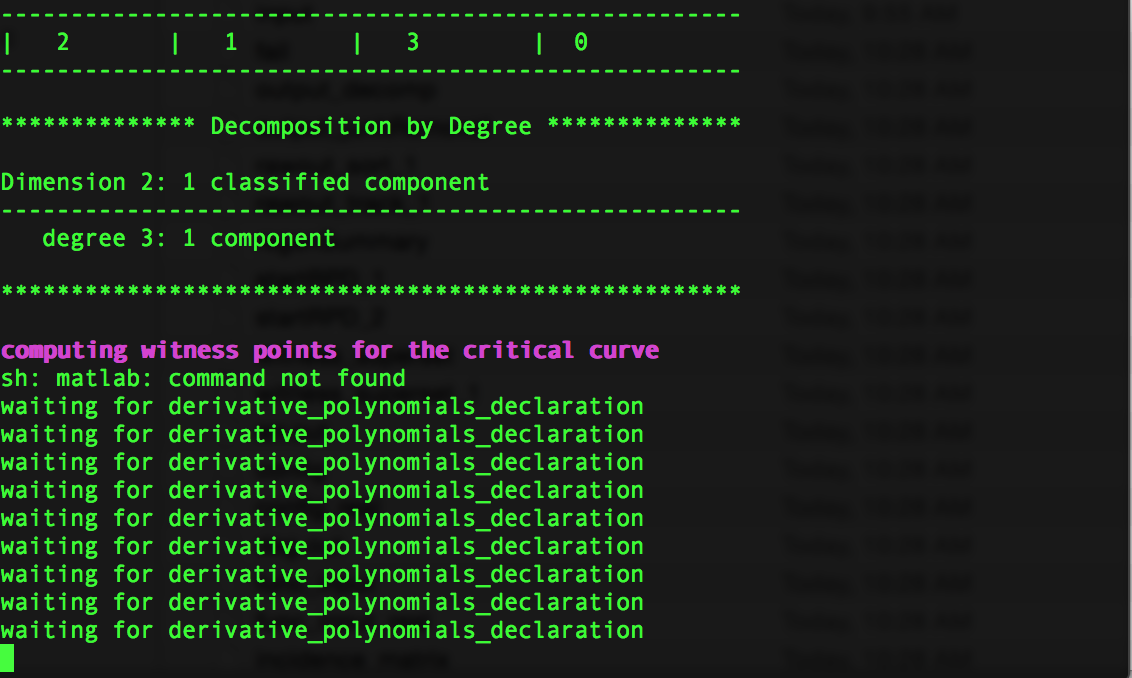
\includegraphics[width=0.6\textwidth]{MATLABExecutableFailure}
\end{minipage}\end{center}

Permanently fixing this error involves editing your profile, e.g. \texttt{bash\_profile}. From your home directory, open \texttt{.bash\_profile} and add the following line: \texttt{export \gls{path}=/PATH/TO/MATLAB.app/bin:\$PATH} where \texttt{PATH/TO/MATLAB.app} points to the location of the Matlab executable. If you do not have, type \texttt{touch .bash\_profile}, which will create \texttt{.bash\_profile}, and then add \texttt{export \gls{path}=/PATH/TO/MATLAB.app/bin:\$PATH}. This should result in the Matlab executable being added to the path whenever opening terminal. 




\subsubsection{Calling Bertini\_real from within Matlab}

Note that you cannot run Bertini\_real from within Matlab, even with the use of {\tt !}, because Bertini\_real currently calls Matlab using a {\tt system()} call. 


\subsubsection*{Removing dependency on Matlab's symbolic toolbox}



Removal of Matlab as a dependency is ongoing work.  Please consider helping me move to Python or another open source language for the symbolic computations, required for deflation of singular curves, and the writing of the input file for critical curves of surfaces.



\section{Examples}

	\subsection{Curves}

	\subsection{Surfaces}



\clearpage
\bibliographystyle{plain}
\bibliography{br_refs}




\appendix


%%%%%%%%%%%%%%%%%%
%
%  APPENDICES
%
%%%%%%%%%%%%%%%%%%



\section{Install}


\label{sec:installation}
	This section of the manual focuses on how to install the necessary dependencies and programs needed to run Bertini\_real on a user's computer. The instructions provided describe the process for Linux, Mac, and Windows operating systems. If you want to try to port Bertini\_real to another operating system, please contact Daniel Brake. 

	When installing Bertini\_real, there are a number of steps required in order to successfully install and run the program. They are:
\begin{enumerate}
\item Installing the \glspl{dependent}
\item Installing Bertini
\item Installing Bertini\_real
\end{enumerate}




\subsection{Dependencies}

Before installing Bertini and Bertini\_real, there are a number of packages that need to be installed. The method used to install these \glspl{dependent} changes depending on the operating system, so please be sure to read the section that describes your particular system.
The dependencies are: 
\begin{itemize}
\item a C++ compiler capable of the C++ 11 standard
\item an \gls{mpi} (such as MPICH2)
\item Boost $>$= 1.53
\item \gls{mpfr}
\item \gls{gmp}
\end{itemize} \cite[p.~4]{Br15}

	\subsubsection*{MATLAB}
The program MATLAB also needs to be installed on your computer as well. Instructions on how to install the program are not provided here. However, if you are associated with a university, or a research facility, they probably have download instructions on their technology support website (e.g. Notre Dame's OIT website). 

\subsubsection*{In Windows}

After installing MATLAB, please be sure to add \texttt{C:\textbackslash{User}\textbackslash{username}\textbackslash{\ldots}\textbackslash{matlab.exe}} to your PATH variable. 


\subsubsection*{In Unix \ GNU Linux}

If you do not already have MATLAB on the PATH, type \texttt{touch .bash\_profile}, which will create \texttt{.bash\_profile}, and then add \texttt{export PATH=/PATH/TO/MATLAB.app/bin:\$PATH}. This should result in the MATLAB executable being added to the path whenever opening terminal. 

If you are a Windows user, the instructions on had to add MATLAB to the \gls{path} are included in the Windows Instructions section


	\subsection{Instructions for GNU/Linux}

Use the package manager provided, such as apt-get, to install the dependencies into your preferred directory.

	\subsection{Instructions for OSX}

  \subsubsection{Preliminary Work}
  \begin{itemize}
    \item Download XCode 8 from the App Store to access its software development tools
    \begin{enumerate}
      \item In terminal, type `'xcode - select -- install`' (open XCode first before doing this)
    \end{enumerate}  
    \item It is recommended that Mac users install the program \href{http://brew.sh}{Homebrew} to use to install these packages. Once that has been done, installing the previously listed dependencies becomes simple. In terminal,  type \texttt{brew search \_\_\_\_} to list packages related to \_\_\_\_, where \_\_\_\_ is your search (for example, GMP, Boost, or MPICH2). To download via Homebrew, type in terminal \texttt{brew install \_\_\_\_}
     \begin{enumerate}
      \item Run it in the terminal
      \item Use directions from website on how to install it
      \item Authenticate it
     \end{enumerate}  
     \item Matlab: make sure to have it installed
  \end{itemize}

  \subsubsection{Installation}
  \begin{itemize}
    \item Install Bertini 1.5.1 (or latest version) from source
     \begin{enumerate}
      \item Make sure to download the source tarball (.tar.gz) from \href{http://bertini.nd.edu}{Bertini}
      \item Unpack the tarball (Double Click)
      \item Now use homebrew to install dependencies for Bertini1 (`brew install autoconf automake libtool mpfr gmp boost mpich`)
      \item In the terminal, move to the unpacked tarball for Bertini1
      \item `./configure`
      \item `make -j 4 && make install`
    \end{enumerate}
    \item Get the source code for Bertinireal  
     \begin{enumerate}
      \item `which git`  if it's emtpy, then `brew install git`
      \item `mkdir code && cd code`
      \item `git clone git://github.com/ofloveandhate/bertini\_real`
      \item `cd bertini\_real`
      \item `autoreconf -i`
      \item `./configure`
      \item `make -j 4 && make install` 
     \end{enumerate} 
  \end{itemize}  


	\subsection{Instructions for Windows}
Unlike Linux or Mac computers, Windows users have additional pre-requisites that they need to install in order to use Bertini and Bertini\_real- they need to first install the program Cygwin.  Alternatively, with Windows 10 and Bash support upcoming, consider using Chocolatey or bash itself.

	\subsubsection{Cygwin}
Cygwin is a Linux- like environment for Windows. The other two operating systems that were discussed above were developed with Linux, while Windows was not. So, in order to run applications like Bertini that need Linux, there needs to be a program or environment that provides Linux for the applications that need it. 

	\paragraph*{How to Install Cygwin}

Cygwin can be found at \href{https://cygwin.com/install.html}{cygwin.com}. Please make sure to choose the version (either 32-bit or 64-bit) that is appropriate for your laptop. After the setup-x86.exe (or setup-x86\_64.exe) have downloaded, run the application, and follow the instructions.

\begin{longtabu} to \textwidth {
    X[1,c]
    X[1,c]}
\hline
\rowfont\bfseries
\textbf{Instructions} & \textbf{Screen Shot} \\
\hline  \\
\endfirsthead
\caption[]{\textit{Continued from previous page}}\\
\hline
\textbf{Instructions} & \textbf{Screen Shot} \\
\hline \\
\endhead
\bottomrule \multicolumn{2}{r}{\textit{Continued on next page}} \\
\endfoot
\bottomrule \multicolumn{2}{r}{\textit{Cite Source Here}} \\
\endlastfoot
Click `next' on the first screen. & 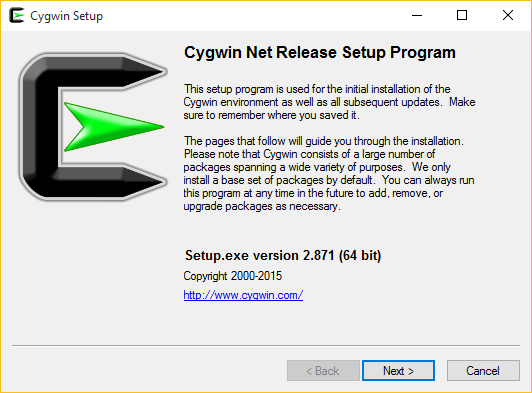
\includegraphics[width=0.4\textwidth]{CygwinInstall1}  \\  \\  \\ 
Select the `Install from Internet' option; click `next'. & 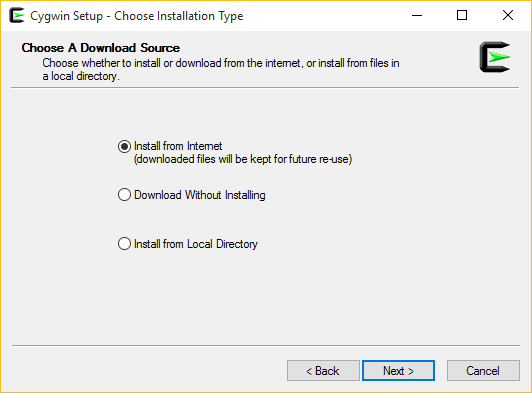
\includegraphics[width=0.4\textwidth]{CygwinInstall2}  \\  \\  \\ 
Enter the preferred installation directory; click `next'. & 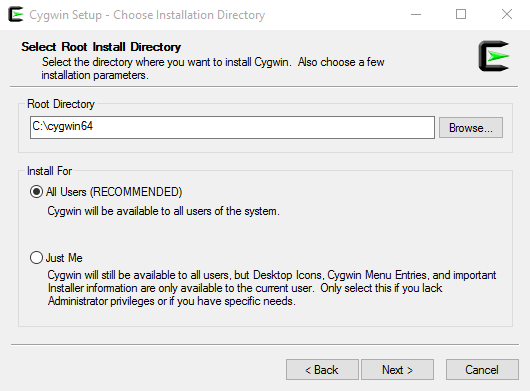
\includegraphics[width=0.4\textwidth]{CygwinInstall3}  \\  \\  \\ 
Choose a temporary installation folder; click `next'. & 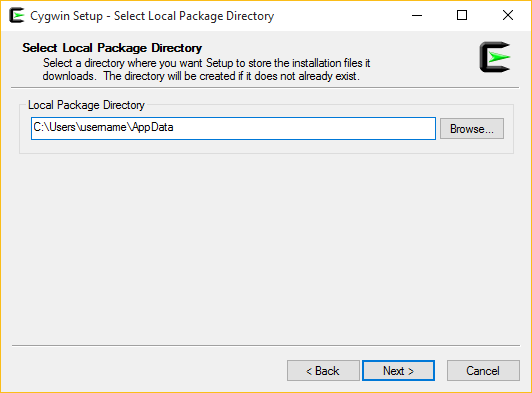
\includegraphics[width=0.4\textwidth]{CygwinInstall4}  \\  \\  \\ 
Select the `Direct Connection' option; click `next'. & 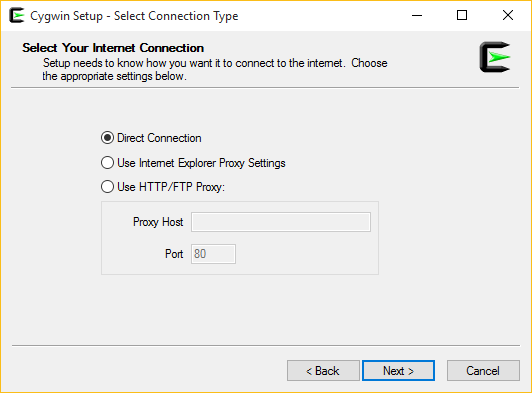
\includegraphics[width=0.4\textwidth]{CygwinInstall5}  \\  \\  \\ 
Choose a download site; click `next'. & 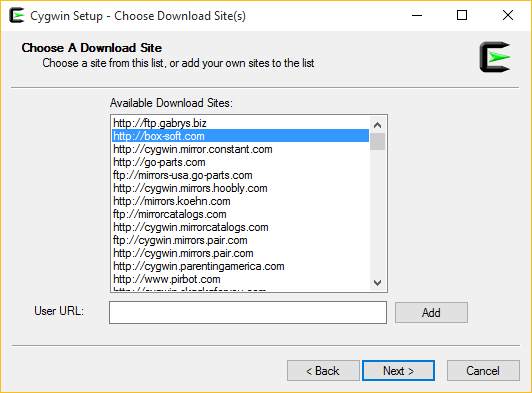
\includegraphics[width=0.4\textwidth]{CygwinInstall6} \\  \\  \\ 
Select the packages that you will need. , then click `next'. See below for more instructions & 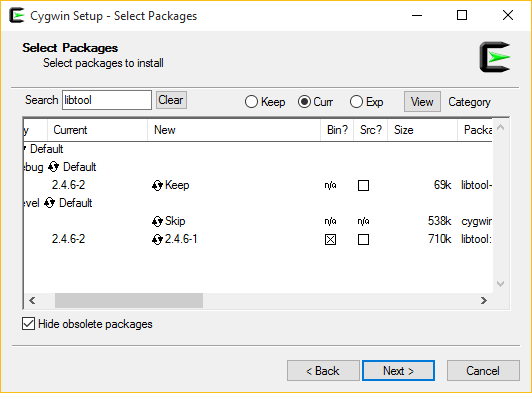
\includegraphics[width=0.4\textwidth]{CygwinInstall7}  \\  \\  \\ 
If during the course of installation, a message pops up and says that certain dependencies are required for the packages, click the `yes' button. When it has installed everything, select `finish'. &  \\  \\   
\end{longtabu}


		\subsubsection*{Selecting packages for Cygwin}
The list of packages that you will need for Bertini\_real can be found below. To find the packages, a user can type the name into the search in the top left of the menu,  which will then show the packages containing that name (e.g. `libtool'). To choose a package click on the text that says `Skip' until it changes to a version number (e.g. `2.4.6-1'). 

\begin{tabular}{ l l }
  autoconf & automake \\
  bash & bison \\
  boost (all the C and C++ libraries) & bzip2 \\
  X-11 & emacs (or nano or some other text editor that you prefer) \\
  flex & vim \\
  mingw-gcc-g++-4.7.3-1 & cygutils-X11 \\
  gmp & gcc \\
  mpc & mpfr \\
  libzip2 & xinit \\
   libtool & openmpi \\
  openssl& openssh \\
  tar & \\
\end{tabular}

	\subsection*{Setting up Cygwin}
		\subsubsection*{Initializing Paths}

In order to properly run Cygwin, you need to add Cygwin to the PATH variable. In order to do so, follow these steps:

\begin{enumerate}

\item Open the Control Panel and select `System'.

\item Select the `Advanced System Settings', and then the `Environment Variables' option. 

\item In the window that appears, select the system variable "PATH' and append \texttt{; C:\textbackslash{cygwin}\textbackslash {bin}} to the end of the PATH variable. When you are doing this, you can also append \texttt{; C:\textbackslash{path}\textbackslash{to}\textbackslash{matlab.exe}} to the end of the PATH as well.

\end{enumerate}

	\subsubsection*{Organizing Cygwin}

	Once Cygwin and MATLAB have been added to the PATH variable, you are now ready to open and run Cygwin. For users who are not familiar with Cygwin, a good reference sheet can be found \href{http://faculty.nps.edu/kmsquire/cs2900/cygwin/fwcygwinref.pdf}{here}.

As part of the installation process, Cygwin will automatically configure and install the packages you selected. This is useful, since it saves a lot of time for the user. However, this also allows a Cygwin user to go and be able to automatically use some of these applications, such as `libtoolize'. Libtoolize, one of the packages that was installed with \texttt{setup\-86x.exe} allows a user to set up a shared library format. In other words, a user doesn't have to call each different library; they are already set up and in the same place.

When I set up Cygwin, I created a new folder located in \texttt{\textbackslash{usr}\textbackslash{local}} that would contain any downloaded files from the Internet that would be used with Cygwin.\par

When setting up Cygwin, I found that in order to install the dependencies that are needed for Bertini and Bertini\_real, they had to be downloaded from the Internet. The following instructions describe how to install these dependencies and finish setting up Cygwin, and were paraphrased from \href{http://cygwin.wikia.com/wiki/How_to_install_GCC_4.3.0}{How to Install a Newer Version of GCC}.

	\subsubsection*{Installing Dependencies}
As stated earlier, the dependencies that need to be downloaded are: 

\begin{tabular}{ l r c }
  C++ compiler & gcc(Cygwin) & \checkmark \\
  MPI & openmpi(Cygwin) & \checkmark \\
  Boost & boost(Cygwin) & \checkmark \\
  \gls{gmp} & gmp(Cygwin) & \checkmark \\
  \gls{mpfr} & \href{http://www.mpfr.org/index.htm}{here} &  \\
  \gls{mpc} & \href{http://www.multiprecision.org}{here} &  \\
\end{tabular} 

Once you have downloaded the programs from the sites, put the zipped files in the folder that you created in \\ \texttt{\textbackslash{usr}\textbackslash{local}\textbackslash{your\_folder}}. Then, in Cygwin, enter \texttt{your\_folder}. 

	\subsubsection* {Linking Cygwin Environment Paths}
After logging into Cygwin, a user needs to set up their environment paths inside the terminal before they set up the files they downloaded. In order to see how the paths currently are set up, either type the following code into the terminal, or copy it and paste it into the terminal: 

\begin{center}\begin{minipage}{0.9\linewidth}

\begin{lstlisting}[language=c++, caption=Adapted from \cite{installnewerGCC}, captionpos=b]
   echo ;\
   echo LD_LIBRARY_PATH=${LD_LIBRARY_PATH}; \
   echo LIBRARY_PATH=${LIBRARY_PATH}; \
   echo CPATH=${CPATH}; \
   echo PATH=${PATH}; \
   echo   \cite{installnewerGCC}
\end{lstlisting}
\end{minipage}\end{center}

Some things to keep in mind while setting up the environment variables \gls{ldlib}, \gls{lib}, and \gls{cpath}:
\begin{itemize}
\item \textbf{LD\_LIBRARY\_PATH} and \textbf{LIBRARY\_PATH} should contain /usr/local/lib (\textbf{LIBRARY\_PATH} shall not be set on Enterprise Linux Enterprise Linux Server release 5.5 (cartage)) 
\item \textbf{CPATH} should contain /usr/local/include
\item If \textbf{PATH} contains \texttt{c:/windows/system32} (or \texttt{/cygdrive/c/windows/system32}; case-insensitive), it should be after /bin and /usr/bin. Otherwise the scripts will try to run Windows sort.exe instead of the Unix command with the same name.
\end{itemize}

To change or modify the different variables, you can use the code below (or you can change the variables in the Control Panel, as shown earlier): 
\begin{center}\begin{minipage}{0.9\linewidth}

\begin{lstlisting}[language=c++, caption=Adapted from \cite{installnewerGCC}, captionpos=b]
   setenv LD_LIBRARY_PATH /usr/local/lib
   setenv LIBRARY_PATH /usr/local/lib
   setenv CPATH /usr/local/include
\end{lstlisting}
\end{minipage}\end{center}

However, if Cygwin shows a message such as \texttt{-bash: setenv: command not found}, then you need to use the code below: 
\begin{center}\begin{minipage}{0.9\linewidth}

\begin{lstlisting}[language=c++, caption=Adapted from \cite{installnewerGCC}, captionpos=b]
   export LD_LIBRARY_PATH=/usr/local/lib
# Depending on system, LIBRARY_PATH shall not be set - 
#  export LIBRARY_PATH=
   export LIBRARY_PATH=/usr/local/lib
   export CPATH=/usr/local/include
\end{lstlisting}
\end{minipage}\end{center}

	\subsubsection*{Building and Installing Packages}
Now that the environment variables are set up, we can now build and set these packages. 

Perform the following build/install steps for the \textbf{MPFR} and \textbf{MPC} packages \textit{\underline{in that order}}:

\begin{enumerate}

\item cd to your workspace directory (above, e.g., cd \textbf{\texttt{\textbackslash{usr} \textbackslash{local} \textbackslash{your\_folder}}})
\item Extract the tarball using tar (e.g., \textbf{\texttt{tar -xf mpfr-3.1.3.tar.bz2}}). This will create a sub-folder with the source for the given package
cd into that source folder (e.g., \textbf{\texttt{cd mpfr-3.1.3}})
\item Type \textbf{\texttt{libtoolize}} into the command line and press enter. This will add the files, once they have been compiled, to the shared library.
\item Generate {\tt configure}, by running the command {\tt autoreconf -i}.
\item Read the README and/or INSTALL file if present
\item Note that for the current version of \textbf{mpc (0.9)} there is a change that may need to be made to have the build work successfully. You need to edit the line of "mpc.h"

\begin{minipage}{0.9\linewidth}
\centering
    \begingroup
    \texttt{%
    \#if defined(\_\_MPC\_WITHIN\_MPC) \&\& \_\_GMP\_LIBGMP\_DLL}
    to
    \texttt{%
    \#if defined \_\_GMP\_LIBGMP\_DLL}
    \endgroup
\end{minipage}

\item run \textbf{\texttt{./configure}} (this will check the configuration of your system for the purpose of this package)(you also need specify \textbf{\texttt{--enable-static --disable-shared}} when compiling the library)
\item run \textbf{\texttt{make}} (this will build the package; \textbf{\texttt{-j}} can speed things up here)
\item run \textbf{\texttt{make check}} (strongly recommended but optional; this will check that everything is correct)
\item run \textbf{\texttt{make install}} (this will install all the relevant files to the relevant directories)
\item run \textbf{\texttt{make clean}} (optional; this will erase intermediate files - important if you are re-attempting a broken build!)

\end{enumerate}








\clearpage
	\subsection{Installing Bertini and Bertini\_real}

Once all of the dependencies have been installed, now Bertini and Bertini\_real can be installed. The zip file for Bertini can be found
\href{http://bertini.nd.edu/download.html}{here}, while the download site for Bertini\_real can be found
\href{http://www.bertinireal.com/download.html}{there}

Move these downloads to your terminal, and unzip and install the two programs. To unpack the directory, just run \texttt{tar -zxvf FILE\_NAME} into the command line while in the folder that the .tar.gz is located. (For Cygwin users, this means going through the same steps as you did for GMP, MPFR, and MPC.) Be sure to install Bertini \textit{\underline{before}} Bertini\_real!!


	\subsection{Setting up MATLAB}
After you have set up Bertini and Bertini\_real, you probably want to be able to see a 3D rendering of your solutions. In order to do so, go to the GitHub  \href{https://github.com/ofloveandhate/bertini_real/tree/master/matlab_codes}{Bertini\_real site} and download the .zip file. I recommend that a new folder is created and that the zip folder goes inside this `master folder'. Unfortunately, the user also has to download each of the functions that are on the same level as the zip folder- e.g. \texttt{dehomogenize.m}, \texttt{find\_constant\_vars.m}, etc. and save those in the `master folder' as well. Make sure that this `master folder' is linked to the folder where the Bertini and Bertini\_real solutions will be located. Once all of these functions and the zip folder are downloaded and saved, then you will be able to successfully use MATLAB in conjunction with Bertini and Bertini\_real. 

\begin{centering}
Congratulations, you have now made it through the installation process. There are some additional features that can also be installed if you so desire, as well as a practice run in order to verify that everything installed correctly.
\end{centering}



		\subsubsection{Parallel Bertini\_real Installation}

Bertini\_real is parallel enabled, using MPI.  You cannot build Bertini\_real without support for MPI at the current time.   To use multiple processors to decompose a real object, call Bertini\_real as you would any other MPI program: \texttt{mpiexec [options] bertini\_real}.











\subsection{Testrun -- the Cayley Cubic}

Now that everything has been installed, we can now do a test run, to make sure that everything is working properly. To test this program, we will try to generate a Cayley Cubic using the above programs, following a number of steps. The first step is to create an input file. Open up a text editor in your terminal and create a file called \texttt{input}. 

Below is the text for this input file.. A key feature to notice is the second line, where the \texttt{tracktype} configuration is set to 1. This configuration setting is necessary for Bertini\_real to run. 

\begin{center}\begin{minipage}{0.9\linewidth}
\begin{lstlisting}[language=c++, caption={\tt input} for the Cayley Cubic, captionpos=b]
CONFIG 
tracktype:1;

END;
INPUT
variable_group x, y, z;
function f;
f = 4 * (x^2 + y^2 + z^2) + 16*x*y*z - 1;
END;
\end{lstlisting}
\end{minipage}\end{center}

Once the input file is created, we can now run Bertini. Simply navigate in the command line to the directory of the input file and type \texttt{bertini} or \texttt{bertini input}.  You may need to type in the entire pathway to where Bertini is located, if it's not in the same folder, so the command line read \newline \texttt{/cygdrive/path/to/BertiniSource\_v1.5/bertini-serial.exe input}\- \\ \textbf{Cygwin users:} A user may also use \texttt{bertini-serial.exe} (or \texttt{bertini\_parallel.exe}). This will run Bertini, creating the Numerical Irreducible Decomposition needed for Bertini\_real. The following should print to the terminal or shell:

\begin{center}\begin{minipage}{0.9\linewidth}
\centering
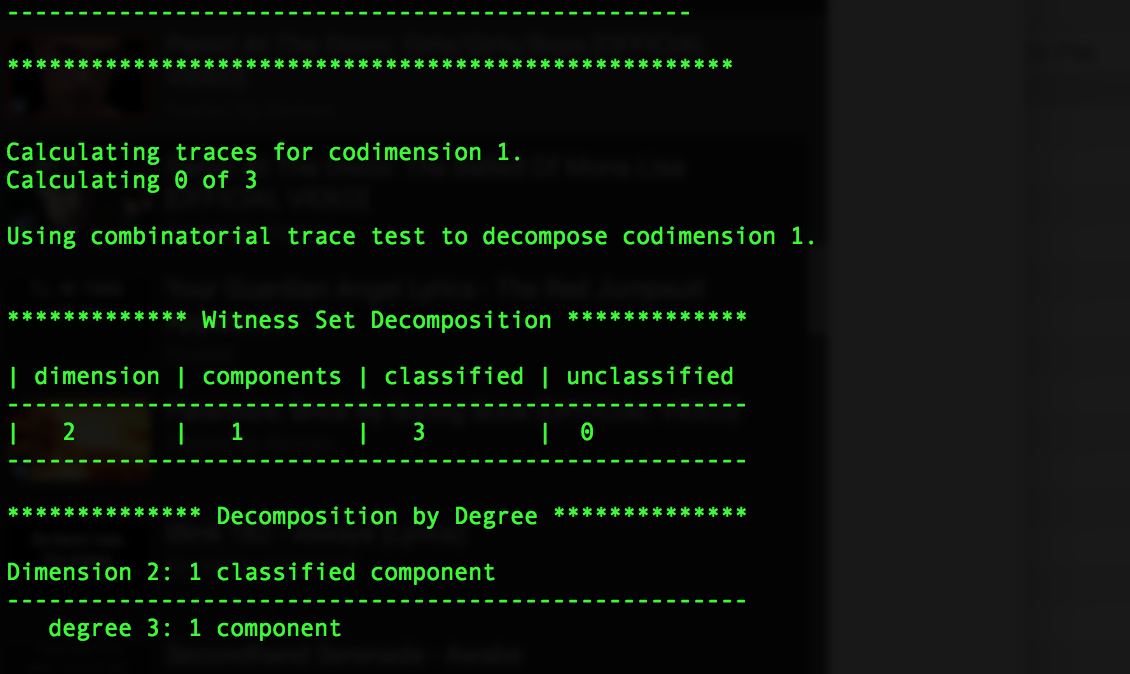
\includegraphics[width=0.6\textwidth]{CayleyCubicBertiniRun.png}
\end{minipage}\end{center}

Once Bertini is finished, the output can be verified as satisfactory (or not). Then, Bertini\_real can be run by calling \texttt{bertini\_real} in the command line. Cygwin users, the same rules that applied to Bertini also apply to Bertini\_real, so be sure to include that `.exe' at the end! However, if the input file used was named `input', no file name is needed at the end of the command line. This program should run for roughly 20-30 seconds, with the final terminal/shell output appearing below:

\begin{center}\begin{minipage}{0.9\linewidth}
\centering
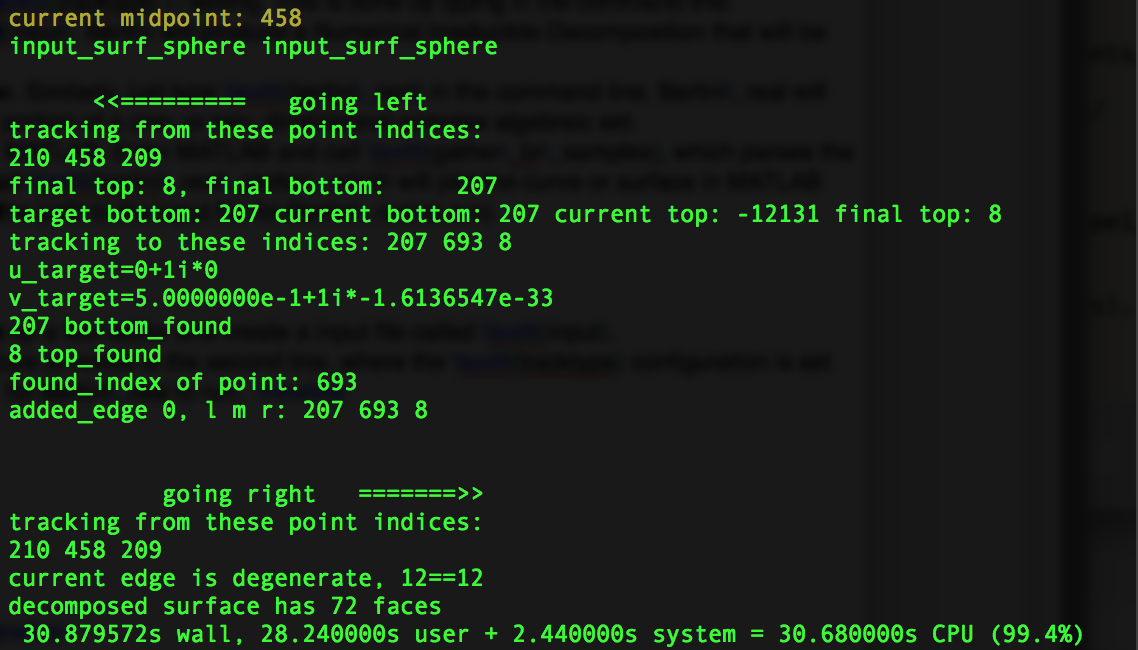
\includegraphics[width=0.6\textwidth]{CayleyCubicBertiniRealRun}
\end{minipage}\end{center}

Finally, MATLAB can be used to visualize the result from the Bertini\_real run. Open MATLAB and enter the `master file', which must be linked to the folder where the Bertini\_real solutions are located. This can be done by first making sure that you are currently in the `master folder', then typing \texttt{addpath(`C:\textbackslash{cygwin64}\textbackslash{path}\textbackslash{to}\textbackslash{solutions\_folder}')} into the command window and pressing enter. Then you can call \texttt{gather\_br\_samples} in the command window, which generates a .mat file. Then, call \texttt{bertini\_real\_plotter\-}. This will create a MATLAB figure, pictured below.

\begin{center}\begin{minipage}{0.9\linewidth}
\centering
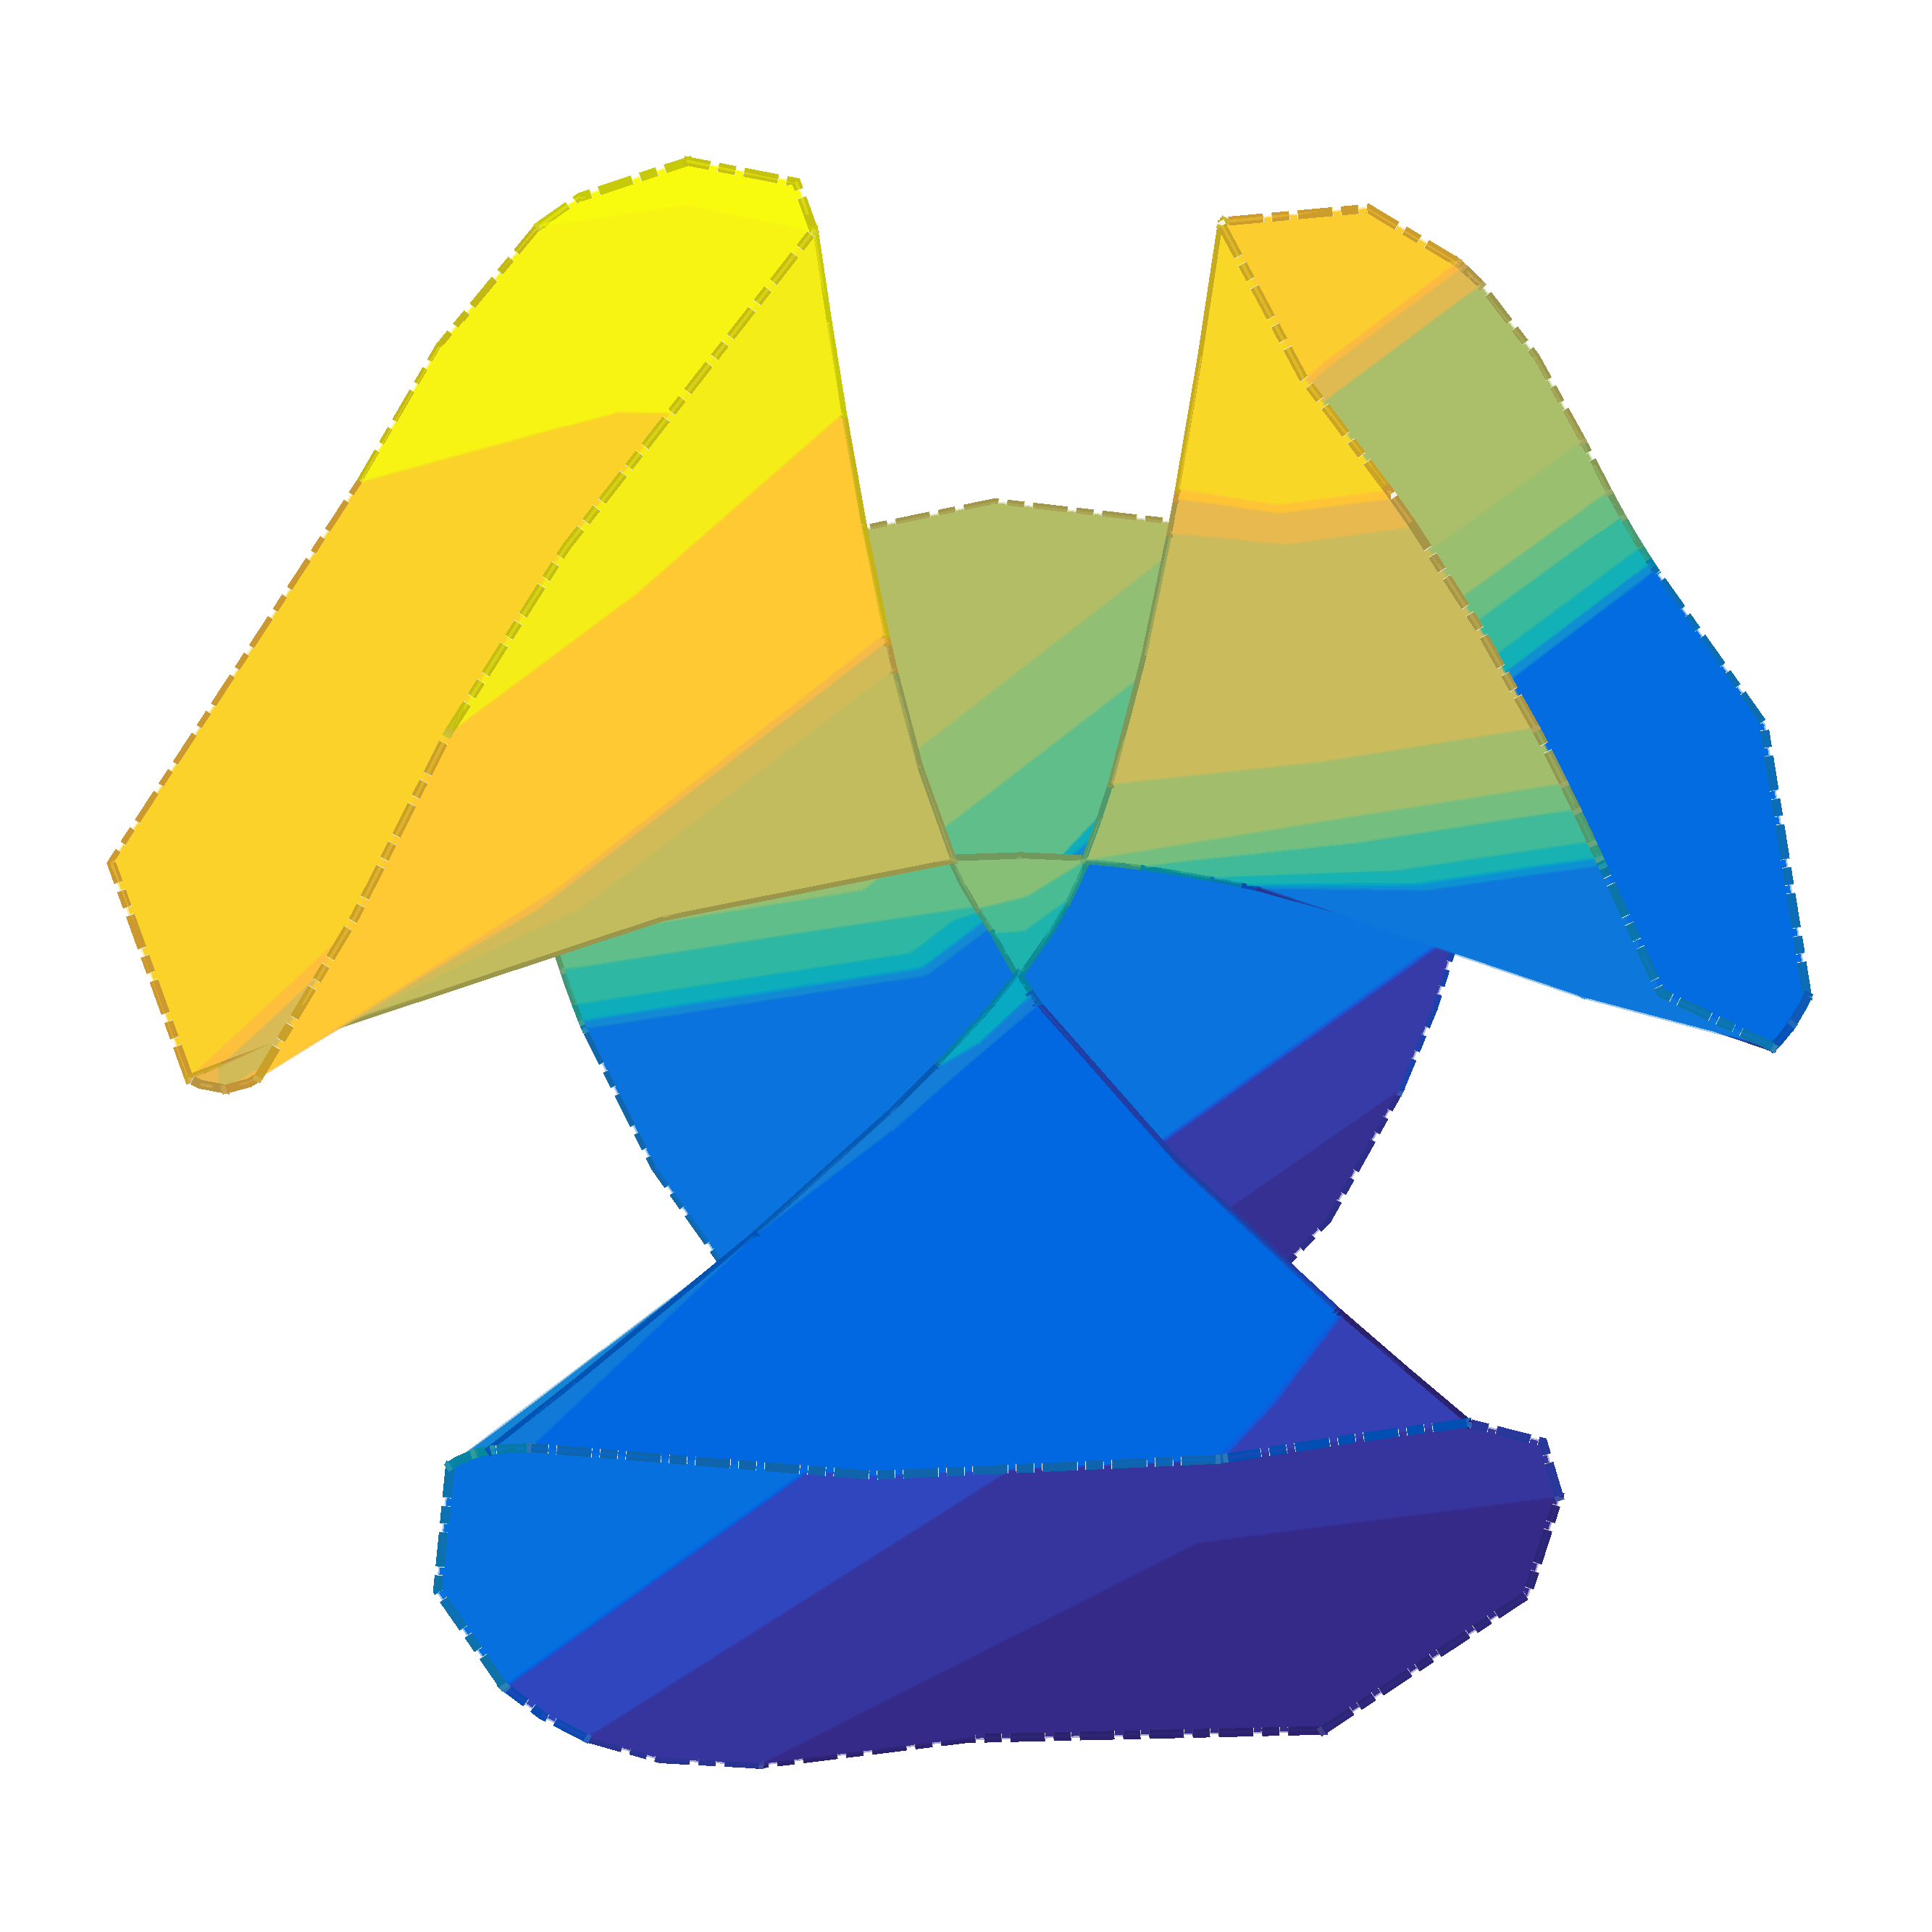
\includegraphics[width=0.6\textwidth]{CayleyCubic}
\end{minipage}\end{center}


If you've been able to reproduce the above figure, then you've mastered the basics of Bertini\_real. 





	\subsection{Other Operating Systems}
If you would like to use Bertini\_real on operating systems that haven't been listed in this manual, please contact Daniel Brake to discuss porting Bertini\_real to your system.






\section{Output Files}
\label{sec:output_files}


In this section, we describe the formats of the plain-text output files from Bertini\_real.
We document abstractly, and let the user explore concretely by generating data.

By default, the output from Bertini\_real is dumped into a folder named {\tt output\_dim\_D\_comp\_C}, where {\tt D} and {\tt C} are the dimension and component numbers.  This can be overridden by specifying option {\tt -o} at runtime.







\subsection{Regardless of dimension}
\label{sec:output_dim_free}

Some files are produced regardless of object dimension:

\begin{itemize}
	\item {\tt decomp} -- \ref{sec:decomp}
	\item {\tt input\_dim\_D\_comp\_C\_deflated} -- a plain copy from Bertini\_real's input in the containing folder.
	\item {\tt run\_metadata} -- \ref{sec:run_metadata}
	\item {\tt V.vertex} -- \ref{sec:v.vertex}
	\item {\tt vertex\_types} -- \ref{sec:vertex_types}
	\item {\tt witness\_data} -- a plain copy from Bertini's output in the containing folder.
	\item {\tt witness\_set} -- \ref{sec:witness_set}
\end{itemize}

Additional important files written NOT into the output folder:
\begin{itemize}
	\item {\tt Dir\_Name} -- \ref{sec:dir_name}
\end{itemize}



\clearpage
\subsubsection{\tt output/decomp}
\label{sec:decomp}



\begin{center}\begin{minipage}{0.9\linewidth}
\begin{lstlisting}[language=c++, caption={\tt output/decomp}, captionpos=b]
input_filename
number_vars dimension // number_vars includes homvar

FOR // # is dimension
	number_vars_in_projection
	FOR
		proj_coord_real proj_coord_imag 
	END FOR
END FOR

number_patches

FOR // # is number_patches
	number_vars_in_patch
	FOR
		patch_coord_real patch_coord_imag 
	END FOR
END FOR

sphere_radius_real sphere_radius_imag
num_sphere_vars  // # is number natural variables
FOR // # is number natural variables
	sphere_center_coord_real sphere_center_coord_imag
END FOR

number_crit_fibers
FOR // # is number_crit_fibers
	crit_fiber_coord_real crit_fiber_coord_imag
END FOR
\end{lstlisting}
\end{minipage}\end{center}


\subsubsection{\tt output/run\_metadata}
\label{sec:run_metadata}

\begin{center}\begin{minipage}{0.9\linewidth}
\begin{lstlisting}[language=c++, caption={\tt output/decomp}, captionpos=b]
bertini_real_version
/path/to/containing/folder
timing statistics from Boost.Chrono
\end{lstlisting}
\end{minipage}\end{center}






\subsubsection{output/V.vertex}
\label{sec:v.vertex}


\begin{center}\begin{minipage}{0.9\linewidth}
\begin{lstlisting}[language=c++, caption={\tt output/V.vertex}, captionpos=b]
num_vertices num_projections  num_variables  num_filenames // number_vars includes homvar

FOR  // num is num_projections
	FOR // num is num coords incl homvar
		proj_coord_real proj_coord_imag
	END FOR
END FOR


FOR  // each filename
	num_chars_in_filename
	filename
END FOR

FOR // each vertex
	num_coords // may include synthetic variables
	FOR
		coord_real coord_imag
	END FOR

	num_projection_values
	FOR
		proj_val_real proj_val_imag
	END FOR

	input_filename_index
	vertex_type  // see file vertex_types
END FOR
\end{lstlisting}
\end{minipage}\end{center}


\subsubsection{output/vertex\_types}
\label{sec:vertex_types}


\begin{center}\begin{minipage}{0.9\linewidth}
\begin{lstlisting}[language=c++, caption={\tt output/vertex\_types}, captionpos=b]
num_vertex_types

FOR
	VertexType value
END FOR
\end{lstlisting}
\end{minipage}\end{center}


Versions of Bertini\_real prior to 1.4
used sequential type indices rather than binary values, to vertex types.  We converted to binary indices to allow vertices to have multiple types, and represent this compactly.  The Matlab visualization code takes advantage of this, and can plot points in each of the type categories they appear in.  The purpose of this file is to let one write code which self-adapts to any future vertex types.







\subsubsection{output/witness\_set}
\label{sec:witness_set}


\begin{center}\begin{minipage}{0.9\linewidth}
\begin{lstlisting}[language=c++, caption={\tt output/witness\_set}, captionpos=b]
num_points dimension component_number

FOR  // each point
	FOR  // each variable
		coord_real coord_imag
	END FOR
END FOR

num_linears num_vars
FOR // each linear
	FOR // each coordinate
		linear_coeff_real linear_coeff_imag
	END FOR
END FOR

num_patches num_vars
FOR // each patch
	FOR // each coordinate
		patch_coeff_real patch_coeff_imag
	END FOR
END FOR


\end{lstlisting}
\end{minipage}\end{center}




\subsubsection{/Dir\_Name}
\label{sec:dir_name}


\begin{center}\begin{minipage}{0.9\linewidth}
\begin{lstlisting}[language=c++, caption={\tt output/V.vertex}, captionpos=b]
/path/to/output/folder
MPType  // why?  I don't know, it seemed important early on.  
dimension 
\end{lstlisting}
\end{minipage}\end{center}

















\clearpage
\subsection{Curve files}
\label{sec:curve_files}

There are several files written for every curve decomposed, into the containing folder.  For surfaces, each sub-curve is written to its own sub-folder, appropriately named.

\begin{itemize}
	\item {\tt output/curve.cnums} -- \ref{sec:curve.cnums}
	\item {\tt output/E.edge} -- \ref{sec:e.edge}
\end{itemize}


\subsubsection{\tt output/curve.cnums}
\label{sec:curve.cnums}


This file contains the cycle numbers of the paths, tracked from the generic midpoint to the left and right points.  Degenerate edges get 0's because there is no path.  Otherwise, the numbers are at least 1.

\begin{center}\begin{minipage}{0.9\linewidth}
\begin{lstlisting}[language=c++, caption={\tt output/curve.cnums}, captionpos=b]
number_edges

FOR // each edge
	going_left going_right
END FOR
\end{lstlisting}
\end{minipage}\end{center}



\subsubsection{\tt output/E.edge}
\label{sec:e.edge}

These are 0-based indices into {\tt V.vertex}.

\begin{center}\begin{minipage}{0.9\linewidth}
\begin{lstlisting}[language=c++, caption={\tt output/E.edge}, captionpos=b]
number_edges

FOR // each edge
	left mid right
END FOR
\end{lstlisting}
\end{minipage}\end{center}









\clearpage
\subsection{Surface files}
\label{sec:surface_files}


\begin{itemize}
	\item {\tt output/F.faces} -- \ref{sec:f.faces}
	\item {\tt output/S.surf} -- \ref{sec:s.surf}
\end{itemize}

\subsubsection{\tt F.faces}
\label{sec:f.faces}
\begin{center}\begin{minipage}{0.9\linewidth}
\begin{lstlisting}[language=c++, caption={\tt output/F.faces}, captionpos=b]
number_faces

FOR // each face
	midpoint
	critslice_index
	top_edge_index bottom_edge_index
	system_name_top system_name_bottom

	num_left_edges
	FOR // each left edge
		edge_index
	END FOR

	num_right_edges
	FOR // each right edge
		edge_index
	END FOR
END FOR
\end{lstlisting}
\end{minipage}\end{center}

\subsubsection{\tt S.surf}
\label{sec:s.surf}

\begin{center}\begin{minipage}{0.9\linewidth}
\begin{lstlisting}[language=c++, caption={\tt output/S.surf}, captionpos=b]
number_faces 0 num_midslices num_critslices

number_singular_curves
FOR // each singular curve
	singcurve_multiplicity index
END FOR
\end{lstlisting}
\end{minipage}\end{center}








\newpage

\begingroup\setlength{\parskip}{0pt plus .1pt}
\setglossarystyle{altlist}
\printglossary[type=\acronymtype]
\endgroup


\printindex

\end{document}
